\part{JavaScript}

\newpage

\chapter{JavaScript简介}

\section{编程简介}

\subsection{编程简介}

程序(program)是为了让计算机执行某些操作或者解决问题而编写的一系列有序指令的集合。由于计算机只能够识别二进制数字0和1,因此需要使用特殊的编程语言来描述如何解决问题过程和方法。 \\

算法(algorithm)是可完成特定任务的一系列步骤,算法的计算过程定义明确,通过一些值作为输入并产生一些值作为输出。 \\

流程图(flow chart)是算法的一种图形化表示方式,使用一组预定义的符号来说明如何执行特定任务。

\begin{itemize}
	\item 圆角矩形:开始和结束
	\item 矩形:数据处理
	\item 平行四边形:输入/输出
	\item 菱形:分支判断条件
	\item 流程线:步骤
\end{itemize}

\begin{figure}
	\centering
	\begin{tikzpicture}[node distance=2cm]
		\node (start) [startend] {Start};
		\node (init)   [io, below of=start] {$ i = 0 $, $ sum = 0 $};
		\node (decision)  [decision, below of=init] {$ i \le 100 $?};
		\node (accumulation) [process, below of=decision] {$ sum = sum + i $};
		\node (update) [process, below of=accumulation] {$ i = i + 1 $};
		\node (output) [io, right of=decision, xshift=2.5cm] {print $ sum $};
		\node (end) [startend, below of=update] {End};

		\draw [arrow] (start) -- (init);
		\draw [arrow] (init) -- (decision);
		\draw [arrow] (decision) -- node[anchor=east] {yes } (accumulation);
		\draw [arrow] (accumulation) -- (update);
		\draw [arrow] (update) -- (-3,-8) -- (-3,-4) -- (decision);
		\draw [arrow] (decision) -- node[anchor=south] {no} (output);
		\draw [arrow] (output) |- (end);
	\end{tikzpicture}
	\caption{计算$ \sum_{i=1}^{100} i $的流程图}
\end{figure}

\subsection{编程语言(Programming Language)}

编程语言主要分为面向机器、面向过程和面向对象三类。JavaScript是一种具有函数优先的轻量级,解释型或即时编译型的编程语言。虽然它是作为开发Web页面的脚本语言而出名,但是它也被用到了很多非浏览器环境中。JavaScript基于原型编程、多范式的动态脚本语言,并且支持面向对象、命令式、声明式、函数式编程范式。

\begin{figure}[H]
	\centering
	
\includegraphics[scale=0.9]{img/C9/9-1/1.png}
	\caption{常见编程语言}
\end{figure}

\section{Hello World!}

\subsection{Hello World!}

使用<script>在HTML网页中插入JavaScript代码。 \\

\begin{lstlisting}[style=htmlcssjs]
<script type="text/JavaScript">
    // JavaScript代码
</script>
\end{lstlisting}

type属性表示在<script>之间的是文本类型,告诉了浏览器里面的文本属于JavaScript语言。 \\

JS作为一种脚本语言可以放在HTML页面中任何位置,但是一般放在网页的<head>或<body>部分。最常用的方式是在页面<head>部分放置<script>元素,浏览器解析HTML时是按先后顺序的,所以前面的<script>就先被执行。 \\

\subsection{引入外部JS文件}

除了在HTML文件中使用<script>添加JS代码,还能把HTML和JS分开,单独创建一个JS文件,其文件后缀为“.js”,然后直接将JS代码写在JS文件中。注意在JS文件中,不需要<script>,直接编写JS代码即可。 \\

JS文件不能直接运行,需要嵌入到HTML文件中执行,因此需要在HTML中引入外部JS文件。 \\

\begin{lstlisting}[style=htmlcssjs]
<script src="JS文件.js"></script>
\end{lstlisting}

\vspace{0.5cm}

\mybox{Hello World!}

\begin{lstlisting}[style=htmlcssjs, title=hello\_world.html]
<!DOCTYPE html>
<html lang="en">
<head>
    <meta charset="UTF-8">
    <title>Hello World!</title>
    <script src="hello_world.js"></script>
</head>
<body>

</body>
</html>
\end{lstlisting}

\begin{lstlisting}[style=htmlcssjs, title=hello\_world.js]
document.write("Hello World!");
\end{lstlisting}

\newpage

\section{语句与注释}

\subsection{语句(Statement)}

JS语句是发给浏览器的命令,这些命令的作用是告诉浏览器要做的事情。一行语句通常在结尾加上一个【;】表示语句的结束,虽然分号也可以不写,但是要养成编程的好习惯,记得在语句末尾加上分号。

\subsection{注释(Comment)}

在编程中加入注释可以增加程序的可读性和可维护性,编译器不会对注释的部分进行编译。 \\

JS中注释分为两类:

\begin{enumerate}
	\item 单行注释:将一行内【//】之后的内容视为注释。
	\item 多行注释:以【/*】开始,【*/】结束,中间的内容视为注释。
\end{enumerate}

\mybox{注释} \\

\begin{lstlisting}[style=htmlcssjs]
document.write("单行注释");     // 我是单行注释
/*
    我是
    多行
    注释
*/
document.write("多行注释");
\end{lstlisting}

\newpage

\section{互动方法}

\subsection{document.write()}

document.write()可用于直接向HTML输出流写内容,简单地说就是直接在网页中输出内容。 \\

\begin{lstlisting}[style=htmlcssjs]
document.write("互动方法:document.write()");
\end{lstlisting}

\subsection{console.log()}

console.log()用于在控制台输出信息,该方法对于开发过程进行测试很有帮助。 \\

\begin{lstlisting}[style=htmlcssjs]
console.log("互动方法:console.log()");
\end{lstlisting}

\subsection{alert()}

在访问网站的时候,有时会突然弹出一个小窗口,上面写着一段提示信息文字,如果不点击“确定”,就不能对网页做任何操作,这个小窗口就是使用alert()实现的。 \\

\begin{lstlisting}[style=htmlcssjs]
alert("互动方法:alert()");
\end{lstlisting}

\subsection{confirm()}

confirm()消息对话框通常用于允许用户做选择的动作,弹出对话框包含一个确定按钮和一个取消按钮。 \\

confirm()的返回值为boolean值,当用户点击“确定”按钮时返回true,当用户点击“取消”按钮时返回false。 \\

\begin{lstlisting}[style=htmlcssjs]
confirm("互动方法:confirm()");
\end{lstlisting}

\subsection{prompt()}

prompt()弹出消息对话框,通常用于询问一些需要与用户交互的信息,弹出的消息对话框包含一个确定按钮、取消按钮和一个文本输入框。 \\

prompt()接受两个参数,第一个参数为要显示在消息对话框中的文本,不可修改;第二个参数为文本框中的内容,可以修改。点击“确定”按钮,文本框中的内容将作为函数的返回值;点击“取消”按钮,将返回null。 \\

\begin{lstlisting}[style=htmlcssjs]
prompt("互动方法:prompt()", "文本内容");
\end{lstlisting}

\newpage

\section{变量}

\subsection{变量(Variable)}

变量是计算机中一块特定的内存空间,由一个或多个连续的字节组成,不同数据存入具有不同内存地址的空间,相互独立,通过变量名可以简单快速地找到在内存中存储的数据。定义变量使用关键字var。 \\

\begin{lstlisting}[style=htmlcssjs]
var variable_name;
\end{lstlisting}

变量名需要符合以下的要求:

\begin{enumerate}
	\item 由字母、数字和下划线组成,第一个字符必须为字母或下划线。
	\item 不能包含除【\_】以外的任何特殊字符,如【\%】、【\#】等。
	\item 不可以使用保留字或关键字。
	\item 准确、顾名思义,不要使用汉语拼音。
\end{enumerate}

关键字是编程语言内置的一些名称,具有特殊的用处和意义。

\begin{table}[H]
	\centering
	\setlength{\tabcolsep}{5mm}{
		\begin{tabular}{|c|c|c|c|c|}
			\hline
			break        & else       & new       & var       & case       \\
			\hline
			finally      & return     & void      & catch     & for        \\
			\hline
			switch       & while      & default   & if        & throw      \\
			\hline
			do           & instanceof & typeof    & abstract  & enum       \\
			\hline
			short        & boolean    & export    & interface & static     \\
			\hline
			extends      & long       & super     & char      & final      \\
			\hline
			synchronized & class      & float     & package   & throws     \\
			\hline
			goto         & private    & transient & debugger  & implements \\
			\hline
			volatile     & double     & import    & public    & delete     \\
			\hline
			in           & try        & int       & byte      & native     \\
			\hline
			const        & protected  &           &           &            \\
			\hline
		\end{tabular}
	}
	\caption{关键字}
\end{table}

\subsection{初始化(Initialization)}

变量可以在定义时初始化,也可以在定义后初始化。 \\

在编程中,【=】不是数学中的“等于”符号,而是表示“赋值”,即将【=】右边的值赋给左边的变量。 \\

\begin{lstlisting}[style=htmlcssjs]
var n = 10;
var wage = 8232.56;
\end{lstlisting}

JS变量虽然也可以不声明直接使用,但是这样不规范。

\newpage

\section{数据类型}

\subsection{数据类型}

JS中变量主要有以下几种类型:

\begin{enumerate}
	\item 数字number:整型、浮点型
	\item 字符串string
	\item 布尔boolean
	\item 空对象null
	\item 未定义undefined
	\item 复杂数据类型:数组Array、对象Object
\end{enumerate}

使用typeof()可以检测一个变量的数据类型。 \\

\mybox{数据类型} \\

\begin{lstlisting}[style=htmlcssjs]
var a = 12;
var b = 3.1415;
var c = "hello";
var d = false;

console.log(typeof(a))
console.log(typeof(b))
console.log(typeof(c))
console.log(typeof(d))
\end{lstlisting}

\begin{tcolorbox}
	\mybox{运行结果}
	\begin{verbatim}
number
number
string
boolean
	\end{verbatim}
\end{tcolorbox}

\subsection{类型转换}

类型转换是把变量从一种类型转换为另一种数据类型。类型转换可以是隐式的,也可以是显式的,通过使用强制类型转换的方法来指定。 \\

\mybox{类型转换} \\

\begin{lstlisting}[style=htmlcssjs]
console.log(Number("123"));
console.log(parseInt("456"));
console.log(parseFloat("78.9"));
console.log(String(123456789));
console.log(Boolean(0));
console.log(Boolean(1));
\end{lstlisting}

\begin{tcolorbox}
	\mybox{运行结果}
	\begin{verbatim}
123
456
78.9
123456789
false
true
	\end{verbatim}
\end{tcolorbox}

\newpage

\section{算术运算符}

\subsection{四则运算}

\begin{table}[H]
	\centering
	\setlength{\tabcolsep}{5mm}{
		\begin{tabular}{|c|c|c|}
			\hline
			\textbf{数学符号} & \textbf{JS符号} & \textbf{含义} \\
			\hline
			$ + $             & +               & 加法          \\
			\hline
			$ - $             & -               & 减法          \\
			\hline
			$ \times $        & *               & 乘法          \\
			\hline
			$ \div $          & /               & 除法          \\
			\hline
			$ \dots\dots $    & \%              & 取模          \\
			\hline
		\end{tabular}
	}
	\caption{四则运算}
\end{table}

JS中除法【/】的意义与数学中不同:

\begin{enumerate}
	\item 当相除的两个运算数都为整型,则运算结果为两个数进行除法运算后的整数部分,例如21 / 5的结果为4。

	\item 如果两个运算数其中至少一个为浮点型,则运算结果为浮点型,如21 / 5.0的结果为4.2。
\end{enumerate}

取模(modulo)【\%】表示求两个数相除之后的余数,如22 \% 3的结果为1;4 \% 7的结果为4。

\subsection{复合赋值运算符}

\begin{table}[H]
	\centering
	\setlength{\tabcolsep}{5mm}{
		\begin{tabular}{|c|c|}
			\hline
			\textbf{运算符} & \textbf{描述}           \\
			\hline
			+=              & a += b等价于a = a + b   \\
			\hline
			-=              & a -= b等价于a = a - b   \\
			\hline
			*=              & a *= b等价于a = a * b   \\
			\hline
			/=              & a /= b等价于a = a / b   \\
			\hline
			\%=             & a \%= b等价于a = a \% b \\
			\hline
		\end{tabular}
	}
	\caption{复合赋值运算符}
\end{table}

\newpage

\section{表达式}

\subsection{字符串连接}

【+】运算符不只代表加法,还可以用于连接两个字符串。 \\

\mybox{字符串连接} \\

\begin{lstlisting}[style=htmlcssjs]
console.log("Hello" + "World");
\end{lstlisting}

\begin{tcolorbox}
	\mybox{运行结果}
	\begin{verbatim}
HelloWorld
	\end{verbatim}
\end{tcolorbox}

\subsection{转义字符}

在一个字符串描述的过程中,有可能会有一些特殊字符的信息。

\begin{table}[H]
	\centering
	\setlength{\tabcolsep}{5mm}{
		\begin{tabular}{|c|c|}
			\hline
			\textbf{转义字符}      & \textbf{描述}                        \\
			\hline
			\lstinline|\\| & 表示一个反斜杠\lstinline|\| \\
			\hline
			\lstinline|\'| & 表示一个单引号\lstinline|'| \\
			\hline
			\lstinline|\"| & 表示一个双引号\lstinline|"| \\
			\hline
			\lstinline|\n| & 换行                                 \\
			\hline
			\lstinline|\t| & 横向制表符                           \\
			\hline
		\end{tabular}
	}
	\caption{转义字符}
\end{table}

\mybox{转义字符} \\

\begin{lstlisting}[style=htmlcssjs]
console.log("全球最大同性交友网站\n\'https://github.com\'");
\end{lstlisting}

\begin{tcolorbox}
	\mybox{运行结果}
	\begin{verbatim}
全球最大同性交友网站
'https://github.com'
	\end{verbatim}
\end{tcolorbox}

\subsection{表达式(Expression)}

表达式与数学中的定义相似,表达式是值具有一定的值,用操作符把常数和变量连接起来的代数式。 \\

使用prompt()可以获取用户输入的信息,返回值为字符串类型。 \\

\mybox{计算圆的面积} \\

\begin{lstlisting}[style=htmlcssjs]
var PI = 3.14159;
var r = parseFloat(prompt("输入半径"));
var area = PI * r ** 2;
console.log("面积 = " + area);
\end{lstlisting}

\begin{tcolorbox}
	\mybox{运行结果}
	\begin{verbatim}
输入半径:5
面积 = 78.53975
	\end{verbatim}
\end{tcolorbox}

Math.floor()的作用是向下取整,Math.ceil()的作用是向上取整。 \\

\mybox{逆序三位数} \\

\begin{lstlisting}[style=htmlcssjs]
var num = parseInt(prompt("输入一个正三位数"));
var a = Math.floor(num / 100);
var b = Math.floor(num / 10) % 10;
var c = num % 10;

num = c * 100 + b * 10 + a;
console.log("逆序:" + num);
\end{lstlisting}

\begin{tcolorbox}
	\mybox{运行结果}
	\begin{verbatim}
输入一个正三位数:520
逆序:25
	\end{verbatim}
\end{tcolorbox}

\newpage

\chapter{判断}

\section{逻辑运算符}

\subsection{关系运算符}

\begin{table}[H]
	\centering
	\setlength{\tabcolsep}{5mm}{
		\begin{tabular}{|c|c|}
			\hline
			\textbf{数学符号} & \textbf{关系运算符} \\
			\hline
			$ < $             & <                   \\
			\hline
			$ > $             & >                   \\
			\hline
			$ \le $           & <=                  \\
			\hline
			$ \ge $           & >=                  \\
			\hline
			$ \ne $           & !=                  \\
			\hline
			$ = $             & ==                  \\
			\hline
		\end{tabular}
	}
	\caption{关系运算符}
\end{table}

\subsection{逻辑运算符}

JS中逻辑运算符有三种:

\begin{enumerate}
	\item 逻辑与\&\&(logical AND):当多个条件同时为真,结果为真。
	      \begin{table}[H]
		      \centering
		      \setlength{\tabcolsep}{5mm}{
			      \begin{tabular}{|c|c|c|}
				      \hline
				      \textbf{条件1} & \textbf{条件2} & \textbf{条件1 \&\& 条件2} \\
				      \hline
				      T              & T              & T                         \\
				      \hline
				      T              & F              & F                         \\
				      \hline
				      F              & T              & F                         \\
				      \hline
				      F              & F              & F                         \\
				      \hline
			      \end{tabular}
		      }
		      \caption{逻辑与}
	      \end{table}

	\item 逻辑或||(logical OR):多个条件有一个为真时,结果为真。
	      \begin{table}[H]
		      \centering
		      \setlength{\tabcolsep}{5mm}{
			      \begin{tabular}{|c|c|c|}
				      \hline
				      \textbf{条件1} & \textbf{条件2} & \textbf{条件1 || 条件2} \\
				      \hline
				      T              & T              & T                       \\
				      \hline
				      T              & F              & T                       \\
				      \hline
				      F              & T              & T                       \\
				      \hline
				      F              & F              & F                       \\
				      \hline
			      \end{tabular}
		      }
		      \caption{逻辑或}
	      \end{table}

	\item 逻辑非!(logical NOT):条件为真时,结果为假;条件为假时,结果为真。
	      \begin{table}[H]
		      \centering
		      \setlength{\tabcolsep}{5mm}{
			      \begin{tabular}{|c|c|}
				      \hline
				      \textbf{条件} & \textbf{!条件} \\
				      \hline
				      T             & F              \\
				      \hline
				      F             & T              \\
				      \hline
			      \end{tabular}
		      }
		      \caption{逻辑非}
	      \end{table}
\end{enumerate}

\newpage

\section{if}

\subsection{if}

当if语句的条件为真时,进入花括号执行内部的代码;若条件为假,则跳过花括号执行后面的代码。 \\

if语句主要有以下几种形式:

\begin{itemize}
	\item 单分支 \\
	      \begin{lstlisting}[style=htmlcssjs]
var age = 15;
if(age > 0 && age < 18) {
    console.log("未成年")
}
        \end{lstlisting}

	\item 双分支 \\
	      \begin{lstlisting}[style=htmlcssjs]
var age = 30;
if(age > 0 && age < 18) {
    console.log("未成年人")
} else {
    console.log("成年人");
}
\end{lstlisting}

	\item 多分支 \\
	      \begin{lstlisting}[style=htmlcssjs]
var score = 76;

if(score >= 90 && score <= 100) {
    console.log("优秀");
} else if(score >= 60 && score < 90) {
    console.log("合格");
} else {
    console.log("不合格");
}
        \end{lstlisting}
\end{itemize}

\subsection{嵌套结构}

if语句也可以嵌套使用: \\

\begin{lstlisting}[style=htmlcssjs]
if(条件1) {
    if(条件2) {
        // code
    }
}
\end{lstlisting}

\vspace{0.5cm}

\mybox{判断整数奇偶} \\

\begin{lstlisting}[style=htmlcssjs]
var num = parseInt(prompt("输入一个正整数"));

if(num > 0) {
    if(num % 2 == 0) {
        console.log(num + "是偶数");
    } else {
        console.log(num + "是奇数");
    }
}
\end{lstlisting}

\begin{tcolorbox}
	\mybox{运行结果}
	\begin{verbatim}
输入一个正整数:66
66是偶数
	\end{verbatim}
\end{tcolorbox}

\newpage

\section{switch}

\subsection{switch}

switch-case结构可以对整数值的表达式进行判断。 \\

\begin{lstlisting}[style=htmlcssjs]
switch(表达式) {
    case label:
        //code
        break;
    // ...
    default:
        //code
        break;
}
\end{lstlisting}

根据表达式的值,跳转到对应的case处进行执行。需要注意的是,当对应的case中的代码被执行完后,并不会跳出switch,而是会继续执行后面的代码,所以需要使用break跳出switch结构。当所有case都不满足表达式的值时,会执行default语句中的代码,相当于if-else结构中的else。 \\

\mybox{根据月份输出对应的英语简写} \\

\begin{lstlisting}[style=htmlcssjs]
var month = parseInt(prompt("输入月份"));

switch(month) {
    case 1:
        console.log("Jan.");
        break;
    case 2:
        console.log("Feb.");
        break;
    case 3:
        console.log("Mar.");
        break;
    case 4:
        console.log("Apr.");
        break;
    case 5:
        console.log("May");
        break;
    case 6:
        console.log("Jun.");
        break;
    case 7:
        console.log("Jul.");
        break;
    case 8:
        console.log("Aug.");
        break;
    case 9:
        console.log("Sep.");
        break;
    case 10:
        console.log("Oct.");
        break;
    case 11:
        console.log("Nov.");
        break;
    case 12:
        console.log("Dec.");
        break;
    default:
        alert("输入有误");
        break;
}
\end{lstlisting}

\begin{tcolorbox}
	\mybox{运行结果}
	\begin{verbatim}
输入月份:5
May
	\end{verbatim}
\end{tcolorbox}

\newpage

\chapter{循环}

\section{自增/自减运算符}

\subsection{自增/自减运算符}

单目运算符中自增++和自减--运算符可以将变量的值加1和减1,但是++和--可以出现在变量之前或之后,即有四种情况:

\begin{enumerate}
	\item 前缀自增
	\item 前缀自减
	\item 后缀自增
	\item 后缀自减
\end{enumerate}

\begin{table}[H]
	\centering
	\setlength{\tabcolsep}{5mm}{
		\begin{tabular}{|c|l|}
			\hline
			\textbf{表达式} & \textbf{含义}        \\
			\hline
			count++         & 执行完所在语句后自增 \\
			\hline
			++count         & 执行所在语句前自增   \\
			\hline
			count--         & 执行完所在语句后自减 \\
			\hline
			--count         & 执行所在语句前自减   \\
			\hline
		\end{tabular}
	}
	\caption{自增/自减运算符}
\end{table}

\newpage

\section{while}

\subsection{while}

在while循环中,当条件满足时重复循环体内的语句。如果条件永远为真,循环会永无止境的进行下去(死循环),因此循环体内要有改变条件的机会。 \\

控制循环次数的方法就是设置循环变量:初值、判断、更新。 \\

while循环的特点是先判断、再执行,所以循环体有可能会进入一次或多次,也有可能一次也不会进入。 \\

\begin{lstlisting}[style=htmlcssjs]
while(条件) {
    // code
}
\end{lstlisting}

\vspace{0.5cm}

\mybox{计算5个人的平均身高} \\

\begin{lstlisting}[style=htmlcssjs]
var height;
var total = 0;
var average;
var i = 1;

while(i <= 5) {
    height = parseFloat(prompt("输入第" + i + "个人的身高"));
    total += height;
    i++;
}

average = total / 5;
console.log("平均身高:" + average);
\end{lstlisting}

\begin{tcolorbox}
	\mybox{运行结果}
	\begin{verbatim}
输入第1个人的身高:160.8
输入第2个人的身高:175.2
输入第3个人的身高:171.2
输入第4个人的身高:181.3
输入第5个人的身高:164
平均身高:170.5
	\end{verbatim}
\end{tcolorbox}

\newpage

\section{do-while}

\subsection{do-while}

do-while循环在进入循环的时候不做检查,而是在执行完一轮循环体的代码之后,再来检查循环的条件是否满足,如果满足则继续下一轮循环,不满足则结束循环,即至少执行一次循环。 \\

do-while循环的主要特点是先执行、再判断。 \\

\begin{lstlisting}[style=htmlcssjs]
do {
    // code
} while(条件);
\end{lstlisting}

\vspace{0.5cm}

\mybox{计算整数位数} \\

\begin{lstlisting}[style=htmlcssjs]
var num = 123;
var n = 0;

do {
    num = Math.floor(num / 10);
    n++;
} while(num != 0);

console.log("位数:" + n);
\end{lstlisting}

\begin{tcolorbox}
	\mybox{运行结果}
	\begin{verbatim}
输入整数:123
位数:3
	\end{verbatim}
\end{tcolorbox}

\subsection{while与do-while区别}

while循环与do-while循环有以下区别:

\begin{enumerate}
	\item 执行顺序不同。

	\item 初始情况不满足循环条件时,while循环一次都不会执行,do-while循环不管任何情况都至少执行一次。

	\item do-while循环的while语句后有【;】。
\end{enumerate}

\begin{figure}[H]
	\centering
	
\includegraphics[scale=0.2]{img/C11/11-3/1.png}
\end{figure}

\mybox{猜数字} \\

\begin{lstlisting}[style=htmlcssjs]
//产生1-100之间的随机数
var answer = Math.floor(Math.random() * 100) + 1;
var num = 0;
var cnt = 0;

do {
    num = parseInt(prompt("猜一个1-100之间的数字"));
    cnt++;
    if(num > answer) {
        alert("猜大了!");
    } else if(num < answer) {
        alert("猜小了!");
    }
} while(num != answer);

alert("猜对了!你一共用了" + cnt + "次猜对!");
\end{lstlisting}

\begin{tcolorbox}
	\mybox{运行结果}
	\begin{verbatim}
猜一个1-100之间的数字:50
猜大了!
猜一个1-100之间的数字:25
猜小了!
猜一个1-100之间的数字:37
猜小了!
猜一个1-100之间的数字:43
猜小了!
猜一个1-100之间的数字:46
猜小了!
猜一个1-100之间的数字:48
猜小了!
猜一个1-100之间的数字:49
猜对了!你一共用了7次猜对!
	\end{verbatim}
\end{tcolorbox}

\newpage

\section{for}

\subsection{for}

for循环有三个表达式,中间用【;】分隔,【;】不可省略。 \\

\begin{lstlisting}[style=htmlcssjs]
for(表达式1; 表达式2; 表达式3) {
    //code
}
\end{lstlisting}

\begin{itemize}
	\item 表达式1通常是为循环变量赋初值,可省略。
	\item 表达式2是循环条件,判断是否继续执行循环,可省略。
	\item 表达式3为更新循环变量的值,可省略。
\end{itemize}

\mybox{计算1-100的累加和} \\

\begin{lstlisting}[style=htmlcssjs]
var sum = 0;
for(var i = 1; i <= 100; i++) {
    sum += i;
}
console.log("累加:" + sum);
\end{lstlisting}

\begin{tcolorbox}
	\mybox{运行结果}
	\begin{verbatim}
累加:5050
	\end{verbatim}
\end{tcolorbox}

\vspace{0.5cm}

\mybox{计算$ 1 + {1 \over 2} + {1 \over 3} + ... + {1 \over n} $} \\

\begin{lstlisting}[style=htmlcssjs]
var n = 10;
var sum = 0;

for(var i = 1; i <= n; i++) {
    sum += 1 / i;
}

console.log(sum);
\end{lstlisting}

\begin{tcolorbox}
	\mybox{运行结果}
	\begin{verbatim}
2.928968
	\end{verbatim}
\end{tcolorbox}

\vspace{0.5cm}

\mybox{斐波那契数列}

\begin{figure}[H]
	\centering
	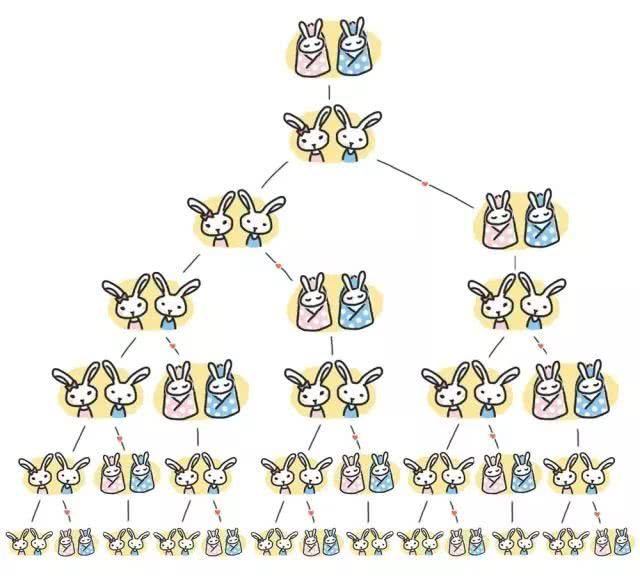
\includegraphics[scale=0.5]{img/C11/11-4/1.png}
\end{figure}

\begin{lstlisting}[style=htmlcssjs]
var n = 10;
var num1, num2, val;
var str = "";

if(n == 1) {
    console.log("1");
} else if(n == 2) {
    console.log("1, 1");
} else {
    num1 = 1;
    num2 = 1;
    str = "1, 1";
    for(var i = 3; i <= n; i++) {
        val = num1 + num2;
        str += ", " + val;
        num1 = num2;
        num2 = val;
    }
    console.log(str);
}
\end{lstlisting}

\begin{tcolorbox}
	\mybox{运行结果}
	\begin{verbatim}
1, 1, 2, 3, 5, 8, 13, 21, 34, 55
	\end{verbatim}
\end{tcolorbox}

\subsection{嵌套循环}

循环也可以进行嵌套使用。 \\

\mybox{九九乘法表} \\

\begin{table}[H]
	\centering
	\setlength{\tabcolsep}{1.5mm}{
		\begin{tabular}{|c|c|c|c|c|c|c|c|c|}
			\hline
			1*1=1 & 1*2=2  & 1*3=3  & 1*4=4  & 1*5=5  & 1*6=6  & 1*7=7  & 1*8=8  & 1*9=9  \\
			\hline
			2*1=2 & 2*2=4  & 2*3=6  & 2*4=8  & 2*5=10 & 2*6=12 & 2*7=14 & 2*8=16 & 2*9=18 \\
			\hline
			3*1=3 & 3*2=6  & 3*3=9  & 3*4=12 & 3*5=15 & 3*6=18 & 3*7=21 & 3*8=24 & 3*9=27 \\
			\hline
			4*1=4 & 4*2=8  & 4*3=12 & 4*4=16 & 4*5=20 & 4*6=24 & 4*7=28 & 4*8=32 & 4*9=36 \\
			\hline
			5*1=5 & 5*2=10 & 5*3=15 & 5*4=20 & 5*5=25 & 5*6=30 & 5*7=35 & 5*8=40 & 5*9=45 \\
			\hline
			6*1=6 & 6*2=12 & 6*3=18 & 6*4=24 & 6*5=30 & 6*6=36 & 6*7=42 & 6*8=48 & 6*9=54 \\
			\hline
			7*1=7 & 7*2=14 & 7*3=21 & 7*4=28 & 7*5=35 & 7*6=42 & 7*7=49 & 7*8=56 & 7*9=63 \\
			\hline
			8*1=8 & 8*2=16 & 8*3=24 & 8*4=32 & 8*5=40 & 8*6=48 & 8*7=56 & 8*8=64 & 8*9=72 \\
			\hline
			9*1=9 & 9*2=18 & 9*3=27 & 9*4=36 & 9*5=45 & 9*6=54 & 9*7=63 & 9*8=72 & 9*9=81 \\
			\hline
		\end{tabular}
	}
	\caption{九九乘法表}
\end{table}

\begin{lstlisting}[style=htmlcssjs]
var str = "";

for(var i = 1; i <= 9; i++) {
    for(var j = 1; j <= 9; j++) {
        str += i + "*" + j + "=" + i*j + "\t";
    }
    str += "\n";
}
console.log(str);
\end{lstlisting}

\vspace{0.5cm}

\mybox{输出图案}

\begin{lstlisting}
*
**
***
****
*****
\end{lstlisting}

\begin{lstlisting}[style=htmlcssjs]
var str = "";

for(var i = 1; i <= 5 i++) {
    for(var j = 1; j <= i; j++) {
        str += "*";
    }
    str += "\n";
}
console.log(str);
\end{lstlisting}

\newpage

\section{break or continue?}

\subsection{循环控制}

循环控制语句的作用是控制当前的循环结构是否继续向下执行,如果不进行控制,那么会根据既定的结构重复执行。如果有一些特殊的情况导致循环的执行中断,就称为循环的控制语句。循环控制语句的关键字有break和continue。 \\

break的作用是跳出当前循环,执行当前循环之后的语句。break只能跳出一层循环,如果是嵌套循环,那么需要按照嵌套的层次,逐步使用break来跳出。break语句只能在循环体内和switch语句内使用。 \\

continue的作用是跳过本轮循环,开始下一轮循环的条件判断。continue终止当前轮的循环过程,但它并不跳出循环。 \\

\mybox{break} \\

\begin{lstlisting}[style=htmlcssjs]
var str = "";

for(var i = 1; i <= 10; i++) {
    if(i == 5) {
        break;
    }
    str += i + " ";
}

console.log(str);
\end{lstlisting}

\begin{tcolorbox}
	\mybox{运行结果}
	\begin{verbatim}
1 2 3 4
	\end{verbatim}
\end{tcolorbox}

\vspace{0.5cm}

\mybox{continue} \\

\begin{lstlisting}[style=htmlcssjs]
var str = "";

for(var i = 1; i <= 10; i++) {
    if(i == 5) {
        continue;
    }
    str += i + " ";
}

console.log(str);
\end{lstlisting}

\begin{tcolorbox}
	\mybox{运行结果}
	\begin{verbatim}
1 2 3 4 6 7 8 9 10
	\end{verbatim}
\end{tcolorbox}

\newpage

\chapter{数组}

\section{一维数组}

\subsection{数组(Array)}

一个变量只能存储一个内容,如果需要存储更多数据,就需要使用数组解决问题。一个数组变量可以存放多个数据,数组是一个值的集合,它们共享同一个名字,数组中的每个变量都能被其下标所访问。 \\

\begin{figure}[H]
	\centering
	\begin{tikzpicture}[scale=0.5]
		\draw[-] (0,0) -- (5,0) -- (10,0) -- (15,0) -- (20,0) -- (25,0) -- (25,3) -- (20,3) -- (15,3) -- (10,3) -- (5,3) -- (0,3) -- (0,0);
		\draw[-] (5,0) -- (5,3);
		\draw[-] (10,0) -- (10,3);
		\draw[-] (15,0) -- (15,3);
		\draw[-] (20,0) -- (20,3);

		\draw (2.5,1.5) node {a[0]};
		\draw (7.5,1.5) node {a[1]};
		\draw (12.5,1.5) node {a[2]};
		\draw (17.5,1.5) node {a[3]};
		\draw (22.5,1.5) node {a[4]};
	\end{tikzpicture}
\end{figure}

\begin{itemize}
	\item 元素:数组中的每个变量
	\item 大小:数组的容量
	\item 下标 / 索引(index):元素的位置,下标从0开始,必须为非负整数
\end{itemize}

使用数组之前首先要创建数组,数组的创建有2种方式:

\begin{enumerate}
	\item 直接创建 \\
	      \begin{lstlisting}[style=htmlcssjs]
var arr1 = [];          //创建一个空数组
var arr2 = [1, 2, 3];   //创建有内容的数组
        \end{lstlisting}

	\item 利用构造函数创建 \\
	      \begin{lstlisting}[style=htmlcssjs]
var arr1 = new Array();                 //创建空数组
var arr2 = new Array(10);               //创建长度为10的数组
var arr3 = new Array(5, 4, 3, 2, 1);    //创建数组并初始化
                \end{lstlisting}
\end{enumerate}

虽然创建数组时指定了长度,但实际上数组都是变长的,也就是说即使指定了长度,仍然可以将元素存储在规定长度以外。

\subsection{数组初始化}

很多时候在使用数组之前需要将数组的内容全部清空,这可以利用循环来实现。 \\

\begin{lstlisting}[style=htmlcssjs]
var arr = new Array(100);
for(var i = 0; i < arr.length; i++) {
    arr[i] = 0;
}
\end{lstlisting}

\vspace{0.5cm}

\mybox{数组最大值和最小值} \\

\begin{lstlisting}[style=htmlcssjs]
var num = [7, 6, 2, 9, 3, 1, 4, 0, 5, 8];
var max = num[0];
var min = num[0];

for(var i = 1; i < num.length; i++) {
    if(num[i] > max) {
        max = num[i];
    } else if(num[i] < min) {
        min = num[i];
    }
}

console.log("max = " + max);
console.log("min = " + min);
\end{lstlisting}

\begin{tcolorbox}
	\mybox{运行结果}
	\begin{verbatim}
max = 9
min = 0
	\end{verbatim}
\end{tcolorbox}

\newpage

\section{二维数组}

\subsection{二维数组(2D Array)}

二维数组包括行和列两个维度,可以看成是由多个一维数组组成。

\begin{table}[H]
	\centering
	\setlength{\tabcolsep}{5mm}{
		\begin{tabular}{|c|c|c|c|}
			\hline
			a[0][0] & a[0][1] & a[0][2] & a[0][3] \\
			\hline
			a[1][0] & a[1][1] & a[1][2] & a[1][3] \\
			\hline
			a[2][0] & a[2][1] & a[2][2] & a[2][3] \\
			\hline
		\end{tabular}
	}
\end{table}

\mybox{直接创建二维数组} \\

\begin{lstlisting}[style=htmlcssjs]
var arr = [[1, 2], [3, 4]];
console.log(arr);
\end{lstlisting}

\begin{tcolorbox}
	\mybox{运行结果}
	\begin{verbatim}
(2) [Array(2), Array(2)]
0: (2) [1, 2]
1: (2) [3, 4]
length: 2
	\end{verbatim}
\end{tcolorbox}

\vspace{0.5cm}

\mybox{构造函数创建二维数组} \\

\begin{lstlisting}[style=htmlcssjs]
var arr = new Array(3);
for(var i = 0; i < arr.length; i++) {
    arr[i] = new Array(4);
}
\end{lstlisting}

\begin{tcolorbox}
	\mybox{运行结果}
	\begin{verbatim}
(3) [Array(4), Array(4), Array(4)]
0: (4) [empty× 4]
1: (2) [empty× 4]
2: (4) [empty× 4]
length: 3
	\end{verbatim}
\end{tcolorbox}

利用两层循环来初始化二维数组。 \\

\mybox{初始化二维数组} \\

\begin{lstlisting}[style=htmlcssjs]
var arr = new Array(3);
for(var i = 0; i < arr.length; i++) {
    arr[i] = new Array(4);
    for(var j = 0; j < arr[i].length; j++) {
        arr[i][j] = 0;
    }
}
\end{lstlisting}

\vspace{0.5cm}

\mybox{矩阵运算} \\

矩阵的加法/减法是指两个矩阵把其相对应元素进行加减的运算。 \\

矩阵加法:两个$ m \times n $矩阵A和B的和,标记为$ A + B $,结果为一个$ m \times n $的矩阵,其内的各元素为其相对应元素相加后的值。 \\

矩阵减法:两个$ m \times n $矩阵A和B的差,标记为$ A - B $,结果为一个$ m \times n $的矩阵,其内的各元素为其相对应元素相减后的值。

\begin{align}\nonumber
	\left[\begin{matrix}
			1 & 3 \\
			1 & 0 \\
			1 & 2 \\
		\end{matrix} \right]
	+
	\left[\begin{matrix}
			0 & 0 \\
			7 & 5 \\
			2 & 1 \\
		\end{matrix} \right]
	=
	\left[\begin{matrix}
			1+0 & 3+0 \\
			1+7 & 0+5 \\
			1+2 & 2+1 \\
		\end{matrix} \right]
	=
	\left[\begin{matrix}
			1 & 3 \\
			8 & 5 \\
			3 & 3 \\
		\end{matrix} \right]
\end{align}

\begin{align}\nonumber
	\left[\begin{matrix}
			1 & 3 \\
			1 & 0 \\
			1 & 2 \\
		\end{matrix} \right]
	-
	\left[\begin{matrix}
			0 & 0 \\
			7 & 5 \\
			2 & 1 \\
		\end{matrix} \right]
	=
	\left[\begin{matrix}
			1-0 & 3-0 \\
			1-7 & 0-5 \\
			1-2 & 2-1 \\
		\end{matrix} \right]
	=
	\left[\begin{matrix}
			1  & 3  \\
			-6 & -5 \\
			-1 & 1  \\
		\end{matrix} \right]
\end{align}

\begin{lstlisting}[style=htmlcssjs]
var A = [
    [1, 3],
    [1, 0],
    [1, 2]
];
    
var B = [
    [0, 0],
    [7, 5],
    [2, 1]
];

var C = new Array(3);
for (var i = 0; i < C.length; i++) {
    C[i] = new Array(2);
}

for(var i = 0; i < C.length; i++) {
    for (var j = 0; j < C[i].length; j++) {
        C[i][j] = A[i][j] + B[i][j];
    }
}
console.log("矩阵加法:" + C);

for(var i = 0; i < C.length; i++) {
    for(var j = 0; j < C[i].length; j++) {
        C[i][j] = A[i][j] - B[i][j];
    }
}
console.log("矩阵减法:" + C);
\end{lstlisting}

\begin{tcolorbox}
	\mybox{运行结果}
	\begin{verbatim}
矩阵加法:[ [ 1, 3 ], [ 8, 5 ], [ 3, 3 ] ]
矩阵减法:[ [ 1, 3 ], [ -6, -5 ], [ -1, 1 ] ]
	\end{verbatim}
\end{tcolorbox}

\newpage

\section{数组操作}

\subsection{计算数组长度}

引用数组的length属性获取数组长度,需要注意的是,JS数组的length属性是可变的。 \\

\mybox{计算数组长度} \\

\begin{lstlisting}[style=htmlcssjs]
var arr = [0, 1, 2, 3, 4];
console.log(arr.length);
arr.length = 10;
console.log(arr.length);
\end{lstlisting}

\begin{tcolorbox}
	\mybox{运行结果}
	\begin{verbatim}
5
10
	\end{verbatim}
\end{tcolorbox}

\subsection{增加元素}

使用下一个未使用的索引,任何时刻可以不断向数组增加新元素。 \\

\mybox{增加元素} \\

\begin{lstlisting}[style=htmlcssjs]
var arr = [0, 1, 2, 3, 4];
arr[5] = 5;
console.log(arr);
\end{lstlisting}

\begin{tcolorbox}
	\mybox{运行结果}
	\begin{verbatim}
[0, 1, 2, 3, 4, 5]
	\end{verbatim}
\end{tcolorbox}

使用unshift()可以向数组第一个元素前面添加一个元素,返回值为数组长度。 \\

\mybox{unshift()} \\

\begin{lstlisting}[style=htmlcssjs]
var arr = [0, 1, 2, 3, 4];
arr.unshift(5);
console.log(arr);
\end{lstlisting}

\begin{tcolorbox}
	\mybox{运行结果}
	\begin{verbatim}
[5, 0, 1, 2, 3, 4]
	\end{verbatim}
\end{tcolorbox}

push()可以向数组最后一个元素后面添加一个元素,返回值为数组长度。 \\

\mybox{push()} \\

\begin{lstlisting}[style=htmlcssjs]
var arr = [0, 1, 2, 3, 4];
arr.push(5);
console.log(arr);
\end{lstlisting}

\begin{tcolorbox}
	\mybox{运行结果}
	\begin{verbatim}
[0, 1, 2, 3, 4, 5]
	\end{verbatim}
\end{tcolorbox}

\subsection{删除元素:}

shift()可以删除数组的第一个元素,返回值为被删除元素。 \\

\mybox{shift()} \\

\begin{lstlisting}[style=htmlcssjs]
var arr = [0, 1, 2, 3, 4];
arr.shift();
console.log(arr);
\end{lstlisting}

\begin{tcolorbox}
	\mybox{运行结果}
	\begin{verbatim}
[1, 2, 3, 4]
	\end{verbatim}
\end{tcolorbox}

pop()可以删除数组的最后一个元素,返回值为被删除元素。 \\

\mybox{pop()} \\

\begin{lstlisting}[style=htmlcssjs]
var arr = [0, 1, 2, 3, 4];
arr.pop();
console.log(arr);
\end{lstlisting}

\begin{tcolorbox}
	\mybox{运行结果}
	\begin{verbatim}
[0, 1, 2, 3]
	\end{verbatim}
\end{tcolorbox}

\subsection{合并数组}

使用concat()可以合并两个或多个数组,该方法不会改变原有数组,而是返回一个新的合并完的数组。 \\

\mybox{concat()} \\

\begin{lstlisting}[style=htmlcssjs]
var arr1 = [1, 2, 3, 4, 5];
var arr2 = [6, 7, 8, 9, 10];
console.log(arr1.concat(arr2));
console.log(arr1);
console.log(arr2);
\end{lstlisting}

\begin{tcolorbox}
	\mybox{运行结果}
	\begin{verbatim}
[1, 2, 3, 4, 5, 6, 7, 8, 9, 10]
[1, 2, 3, 4, 5]
[6, 7, 8, 9, 10]
	\end{verbatim}
\end{tcolorbox}

\subsection{数组转字符串}

使用join(separator)方法可以将数组转换为字符串,其中`separator`参数可选,用于指定要使用的分隔符,如果该参数省略,则使用逗号作为分隔符。 \\

\mybox{join()} \\

\begin{lstlisting}[style=htmlcssjs]
var arr = [0, 1, 2, 3, 4];
console.log(arr.join());
\end{lstlisting}

\begin{tcolorbox}
	\mybox{运行结果}
	\begin{verbatim}
0,1,2,3,4
	\end{verbatim}
\end{tcolorbox}

\subsection{字符串转数组}

6. 使用split(separator, n)可以将字符串转换为数组,其中参数separator必选,用于指定将字符串按某个字符切割成若干个子字符串,并以数组的形式返回。参数n可选,用于指定返回的数组的最大长度,如果设置了该参数,返回的子串数量不会多于n;如果没有设置该参数,整个字符串都会被分隔。 \\

\mybox{split()} \\

\begin{lstlisting}[style=htmlcssjs]
var str = "hello HTML hello CSS hello JavaScript";
var arr = str.split(' ');
console.log(arr);
\end{lstlisting}

\begin{tcolorbox}
	\mybox{运行结果}
	\begin{verbatim}
["hello", "HTML", "hello", "CSS", "hello", "JavaScript"]
	\end{verbatim}
\end{tcolorbox}

\subsection{翻转数组}

使用reverse()可以颠倒数组中元素的顺序。 \\

\mybox{reverse()} \\

\begin{lstlisting}[style=htmlcssjs]
var arr = [1, 2, 3, 4, 5];
console.log(arr.reverse());
\end{lstlisting}

\begin{tcolorbox}
	\mybox{运行结果}
	\begin{verbatim}
[5, 4, 3, 2, 1]
	\end{verbatim}
\end{tcolorbox}

\subsection{数组排序}

使用sort(sortfun)可以将数组进行排序,其中参数sortfun可选,用于指定排序规则,而且必须是函数,该参数省略则按照字符编码顺序排序。 \\

\mybox{sort()} \\

\begin{lstlisting}[style=htmlcssjs]
var arr = [98, 1, 21, 8, 12, 2, 10, 25];
arr.sort(function(a, b) {
    return a > b ? 1 : -1;
});
console.log(arr);
\end{lstlisting}

\begin{tcolorbox}
	\mybox{运行结果}
	\begin{verbatim}
[1, 2, 8, 10, 12, 21, 25, 98]
	\end{verbatim}
\end{tcolorbox}

\subsection{数组切片}

使用slice(start, end)可以返回数组中被选定的元素,不包含下标为end的元素。其中参数start必选,用于指定开始位置,如果是负数则从数组尾部开始算起。参数end可选,用于指定结束位置,没有该参数省略,则切分到数组结束为止,如果是负数则从数组尾部开始算起。 \\

\mybox{slice()} \\

\begin{lstlisting}[style=htmlcssjs]
var arr = [0, 1, 2, 3, 4, 5, 6];
console.log(arr.slice(2, 5));
\end{lstlisting}

\begin{tcolorbox}
	\mybox{运行结果}
	\begin{verbatim}
[2, 3, 4]
	\end{verbatim}
\end{tcolorbox}

\subsection{查找元素}

使用indexOf(item, start)可以查找指定元素,如果查找成功则返回该元素的下标,如果查找失败者返回-1。其中参数item必选,用于指定需要查找的元素,参数start可选,用于指定在数组中开始检索的位置,如省略则从第一个元素开始检索。 \\

\mybox{indexOf()} \\

\begin{lstlisting}[style=htmlcssjs]
var arr = [0, 1, 2, 3, 4, 5, 6];
console.log(arr.indexOf(4));
\end{lstlisting}

\begin{tcolorbox}
	\mybox{运行结果}
	\begin{verbatim}
4
	\end{verbatim}
\end{tcolorbox}

\newpage

\chapter{函数}

\section{函数}

\subsection{函数(Function)}

函数执行一个特定的任务,JS提供了大量内置函数,例如alert()用来显示警告对话框、parseInt()用来将字符串转换为整型等。

\begin{figure}[H]
	\centering
	\begin{tikzpicture}[scale=0.5]
		\draw[-] (5,-2) -- (10,-2) -- (10,2) -- (5,2) -- (5,-2);
		\draw[->] (0,0) -- (5,0);
		\draw[->] (10,0) -- (15,0);

		\draw (-2,0) node {Input};
		\draw (17,0) node {Output};
		\draw (7.5,0) node {Function};
	\end{tikzpicture}
	\caption{函数}
\end{figure}

当调用函数时,程序控制权会转移给被调用的函数,当函数执行结束后,函数会把程序序控制权交还给其调用者。

\begin{figure}[H]
	\centering
	\begin{tikzpicture}[]
		\draw (0,4.5) node {Caller};
		\draw[->] (0,4) -- (0,0.5);
		\draw[->] (0,-0.5) -- (0,-4);
		\draw (0,0) node {调用foo()};

		\draw (4,4) node {foo()};
		\draw[->] (4,3) -- (4,0.5);
		\draw[->] (4,-0.5) -- (4,-3);
		\draw (4,0) node {调用bar()};

		\draw (8,3) node {bar()};
		\draw[->] (8,2) -- (8,-2);

		\draw[->] (0.5,0.5) -- (3.5,3);
		\draw[->] (3.5,-3) -- (0.5,-0.5);
		\draw[->] (4.5,0.5) -- (7.5,2);
		\draw[->] (7.5,-2) -- (4.5,-0.5);
	\end{tikzpicture}
	\caption{函数调用}
\end{figure}

函数的定义需要使用关键字function,函数的参数列表包括参数的类型、顺序、数量等信息,参数列表可以为空。 \\

\begin{lstlisting}[style=htmlcssjs]
function funcName(parameterList) {
    // code
}
\end{lstlisting}

\subsection{函数设计方法}

为什么不把所有的代码全部写在一起,还需要自定义函数呢? \\

使用函数有以下好处:

\begin{enumerate}
	\item 避免代码复制,代码复制是程序质量不良的表现
	\item 便于代码维护
	\item 避免重复造轮子,提高开发效率
\end{enumerate}

在设计函数的时候需要考虑以下的几点要素:

\begin{enumerate}
	\item 确定函数的功能

	\item 确定函数的参数
	      \begin{itemize}
		      \item 是否需要参数
		      \item 参数个数
		      \item 参数类型
	      \end{itemize}

	\item 确定函数的返回值
	      \begin{itemize}
		      \item 是否需要返回值
		      \item 返回值类型
	      \end{itemize}
\end{enumerate}

\mybox{函数实现返回最大值} \\

\begin{lstlisting}[style=htmlcssjs]
function max(num1, num2) {
    // if(num1 > num2) {
    //  return num1;
    // } else {
    //  return num2;
    // }

    return num1 > num2 ? num1 : num2;
}

console.log(max(4, 12));
console.log(max(54, 33));
console.log(max(0, -12));
console.log(max(-999, -774));
\end{lstlisting}

\begin{tcolorbox}
	\mybox{运行结果}
	\begin{verbatim}
12
54
0
-774
	\end{verbatim}
\end{tcolorbox}

\vspace{0.5cm}

\mybox{函数实现累加和} \\

\begin{lstlisting}[style=htmlcssjs]
function sum(start, end) {
    var total = 0;
    for(var i = start; i <= end; i++) {
        total += i;
    }
    return total;
}

console.log("1-100的累加和 = " + sum(1, 100));
console.log("1024-2048的累加和 = " + sum(1024, 2048));
\end{lstlisting}

\begin{tcolorbox}
	\mybox{运行结果}
	\begin{verbatim}
1-100的累加和 = 5050
1024-2048的累加和 = 1574400
	\end{verbatim}
\end{tcolorbox}

\vspace{0.5cm}

\mybox{函数实现输出i行j列由自定义字符组成的图案} \\

\begin{lstlisting}[style=htmlcssjs]
function print_chars(row, col, c) {
    var str = "";
    for(var i = 0; i < row; i++) {
        for(var j = 0; j < col; j++) {
            str += c;
        }
        str += "\n";
    }
    console.log(str);
}

print_chars(5, 10, '?');
\end{lstlisting}

\begin{tcolorbox}
	\mybox{运行结果}
	\begin{verbatim}
??????????
??????????
??????????
??????????
??????????
	\end{verbatim}
\end{tcolorbox}

\newpage

\section{局部变量与全局变量}

\subsection{局部变量(Local Varaible)}

JS的局部变量是在函数里面被声明的,这些变量的作用域在本地,也就是说这些变量只能在函数内部可用。本地变量在函数调用时被创造,在函数结束时被销毁。 \\

在函数中,函数的每次调用就会产生一个独立的空间,在这个空间中的变量,是函数的这次运行所独有的,函数的参数也是局部变量。 \\

\mybox{局部变量} \\

\begin{lstlisting}[style=htmlcssjs]
function test(a) {
    a = 2;
    console.log("a = " + a);
}

var a = 1;
console.log("a = " + a);
test(a);
console.log("a = " + a);
\end{lstlisting}

\begin{tcolorbox}
	\mybox{运行结果}
	\begin{verbatim}
a = 1
a = 2
a = 1
	\end{verbatim}
\end{tcolorbox}

\subsection{全局变量(Global Varaible)}

JS的全局变量就是在函数外被声明的变量,作用域为全局,所有的在页面上的脚本和函数都可以获取这些变量。全局变量在其被声明时创建,在页面被关闭时被销毁。 \\

全局变量的优先级低于局部变量,当全局变量与局部变量重名的时候,起作用的是局部变量,全局变量会被暂时屏蔽掉。

\begin{figure}[H]
	\centering
	\begin{tikzpicture}[]
		\draw (4,4.5) node {全局};
		\draw (0,0) rectangle (8,4);

		\draw (2.5,3.5) node {局部};
		\draw (1,1) rectangle (4,3);

		\draw (2.5,2.5) node {变量A};
		\draw (2,1.5) rectangle (3,2);

		\draw (6,2.5) node {变量B};
		\draw (5.5,1.5) rectangle (6.5,2);
	\end{tikzpicture}
	\caption{全局变量}
\end{figure}

\mybox{全局变量} \\

\begin{lstlisting}[style=htmlcssjs]
var a = 1;          // 全局变量

function test() {
    var a = 2;      // 本地变量
    console.log("a = " + a);
}

test();
\end{lstlisting}

\begin{tcolorbox}
	\mybox{运行结果}
	\begin{verbatim}
a = 2
	\end{verbatim}
\end{tcolorbox}

\newpage

\section{递归} \label{recursive}

\subsection{递归(Recursion)}

要理解递归,先得理解递归(见\ref{recursive}章节)。 \\

在函数的内部,直接或者间接的调用自己的过程就叫作递归。对于一些问题,使用递归可以简洁易懂的解决问题,但是递归的缺点是性能低,占用大量系统栈空间。 \\

递归算法很多时候可以处理一些特别复杂、难以直接解决的问题。例如:

\begin{itemize}
	\item 迷宫
	\item 汉诺塔
	\item 八皇后
	\item 排序
	\item 搜索
\end{itemize}

在定义递归函数时,一定要确定一个结束条件,否则会造成无限递归的情况,最终会导致栈溢出。

\begin{figure}[H]
	\centering
	
\includegraphics[scale=0.7]{img/C13/13-3/1.png}
\end{figure}

\begin{figure}[H]
	\centering
	
\includegraphics[scale=0.6]{img/C13/13-3/2.png}
\end{figure}

\begin{figure}[H]
	\centering
	
\includegraphics[scale=0.6]{img/C13/13-3/3.png}
\end{figure}

\begin{figure}[H]
	\centering
	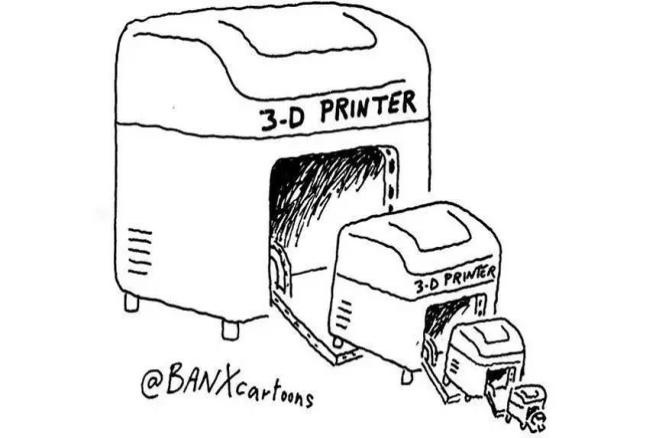
\includegraphics[scale=1.3]{img/C13/13-3/4.png}
\end{figure}

\begin{figure}[H]
	\centering
	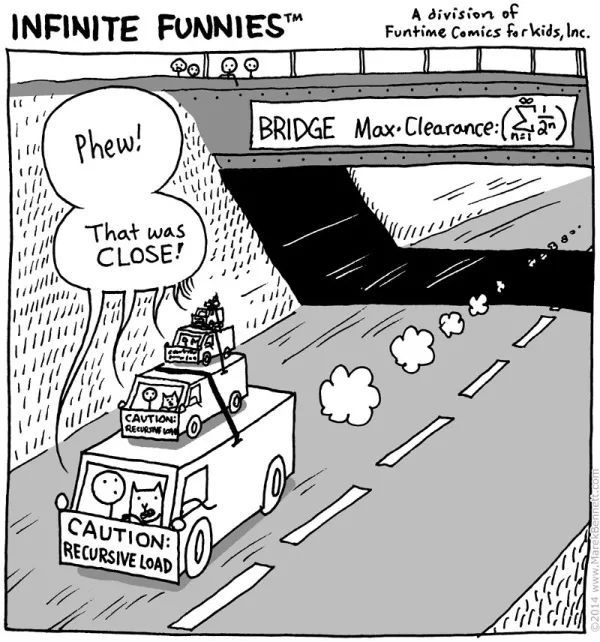
\includegraphics[scale=0.6]{img/C13/13-3/5.png}
\end{figure}

\mybox{无限递归} \\

\begin{lstlisting}[style=htmlcssjs]
function tell_story() {
    console.log("从前有座山");
    console.log("山里有座庙");
    console.log("庙里有个老和尚和小和尚");
    console.log("老和尚对小和尚在讲故事");
    console.log("他讲的故事是:");
    tell_story();
}

tell_story();
\end{lstlisting}

\begin{tcolorbox}
	\mybox{运行结果}
	\begin{verbatim}
从前有座山
山里有座庙
庙里有个老和尚和小和尚
老和尚对小和尚在讲故事
他讲的故事是:
从前有座山
山里有座庙
庙里有个老和尚和小和尚
老和尚对小和尚在讲故事
他讲的故事是:
...
	\end{verbatim}
\end{tcolorbox}

递归函数一般需要定义递归的出口,即结束条件,确保递归能够在适合的地方退出。 \\

\mybox{阶乘} \\

\begin{lstlisting}[style=htmlcssjs]
function factorial(n) {
    if(n == 0 || n == 1) {
        return 1;
    }
    return n * factorial(n - 1);
}

console.log("5! = " + factorial(5));
\end{lstlisting}

\begin{tcolorbox}
	\mybox{运行结果}
	\begin{verbatim}
5! = 120
	\end{verbatim}
\end{tcolorbox}

\begin{figure}[H]
	\centering
	\begin{tikzpicture}[]
		\draw (0,0) rectangle (3,1.5);
		\draw (3,-2) rectangle (6,-0.5);
		\draw (6,-4) rectangle (9,-2.5);
		\draw (9,-6) rectangle (12,-4.5);
		\draw (12,-8) rectangle (15,-6.5);

		\draw (12.75,-10.75) rectangle (14.25,-9.25);
		\draw (9.75,-8.75) rectangle (11.25,-7.25);
		\draw (6.75,-6.75) rectangle (8.25,-5.25);
		\draw (3.75,-4.75) rectangle (5.25,-3.25);
		\draw (0.75,-2.75) rectangle (2.25,-1.25);

		\draw (1.5,0.75) node {$ factorial(5) $};
		\draw (4.5,-1.25) node {$ factorial(4) $};
		\draw (7.5,-3.25) node {$ factorial(3) $};
		\draw (10.5,-5.25) node {$ factorial(2) $};
		\draw (13.5,-7.25) node {$ factorial(1) $};

		\draw (13.5,-10) node {$ 1 $};
		\draw (10.5,-8) node {$ 2 $};
		\draw (7.5,-6) node {$ 6 $};
		\draw (4.5,-4) node {$ 24 $};
		\draw (1.5,-2) node {$ 120 $};

		\draw[->] (3,0.75) -- (4.5,0.75) -- (4.5,-0.5);
		\draw[->] (6,-1.25) -- (7.5,-1.25) -- (7.5,-2.5);
		\draw[->] (9,-3.25) -- (10.5,-3.25) -- (10.5,-4.5);
		\draw[->] (12,-5.25) -- (13.5,-5.25) -- (13.5,-6.5);

		\draw[->] (12.75,-10) -- (10.5,-10) -- (10.5,-8.75);
		\draw[->] (9.75,-8) -- (7.5,-8) -- (7.5,-6.75);
		\draw[->] (6.75,-6) -- (4.5,-6) -- (4.5,-4.75);
		\draw[->] (3.75,-4) -- (1.5,-4) -- (1.5,-2.75);

		\draw (4.5,1) node {$ 5 * factorial(4) $};
		\draw (7.5,-1) node {$ 4 * factorial(3) $};
		\draw (10.5,-3) node {$ 3 * factorial(2) $};
		\draw (13.5,-5) node {$ 2 * factorial(1) $};

		\draw (11,-10.5) node {$ 2 * 1 $};
		\draw (8,-8.5) node {$ 3 * 2 $};
		\draw (5,-6.5) node {$ 4 * 6 $};
		\draw (2,-4.5) node {$ 5 * 24 $};
	\end{tikzpicture}
	\caption{阶乘}
\end{figure}

\mybox{斐波那契数列(递归)} \\

\begin{lstlisting}[style=htmlcssjs]
function fibonacci(n) {
    if(n == 1 || n == 2) {
        return 1;
    }
    return fibonacci(n - 2) + fibonacci(n - 1);
}

n = 7;
console.log("斐波那契数列第" + n + "位:" + fibonacci(7));
\end{lstlisting}

\begin{tcolorbox}
	\mybox{运行结果}
	\begin{verbatim}
斐波那契数列第7位:13
	\end{verbatim}
\end{tcolorbox}

\begin{figure}[H]
	\centering
	\begin{tikzpicture}[
			level distance=2.5cm,
			level 1/.style={sibling distance=6cm},
			level 2/.style={sibling distance=3cm},
			level 3/.style={sibling distance=2cm}
		]
		\node {$ f(5) $}
		child {
				node {$ f(3) $}
				child {node {$ f(1) $}}
				child {
						node {$ f(2) $}
						child {node {$ f(0) $}}
						child {node {$ f(1) $}}
					}
			}
		child {
				node {$ f(4) $}
				child {
						node {$ f(2) $}
						child {node {$ f(0) $}}
						child {node {$ f(1) $}}
					}
				child {
						node {$ f(3) $}
						child {node {$ f(1) $}}
						child {
								node {$ f(2) $}
								child {node {$ f(0) $}}
								child {node {$ f(1) $}}
							}
					}
			};
	\end{tikzpicture}
	\caption{递归树}
\end{figure}

\mybox{斐波那契数列(迭代)} \\

\begin{lstlisting}[style=htmlcssjs]
function fibonacci(n) {
    var f = new Array(n + 1);
    f[1] = f[2] = 1;
    for(var i = 3; i <= n; i++) {
        f[i] = f[i - 2] + f[i - 1];
    }
    return f[n];
}

n = 7;
console.log("斐波那契数列第" + n + "位:" + fibonacci(7));
\end{lstlisting}

\begin{tcolorbox}
	\mybox{运行结果}
	\begin{verbatim}
斐波那契数列第7位:13
	\end{verbatim}
\end{tcolorbox}

\mybox{阿克曼函数}

\begin{align}\nonumber
	A(m, n) =
	\begin{cases}
		n + 1             & m = 0        \\
		A(m-1, 1)         & m > 0, n = 0 \\
		A(m-1, A(m, n-1)) & m > 0, n > 0 \\
	\end{cases}
\end{align}

\begin{lstlisting}[style=htmlcssjs]
function A(m, n) {
    if(m == 0) {
        return n + 1;
    } else if(m > 0 && n == 0) {
        return A(m-1, 1);
    } else if(m > 0 && n > 0) {
        return A(m-1, A(m, n-1));
    }
}

console.log(A(3, 4));
\end{lstlisting}

\begin{tcolorbox}
	\mybox{运行结果}
	\begin{verbatim}
125
	\end{verbatim}
\end{tcolorbox}

\begin{table}[H]
	\centering
	\setlength{\tabcolsep}{0.5mm}{
		\begin{tabular}{|c|c|c|c|c|c|c|}
			\hline
			\diagbox{$ m $}{$ n $} & \textbf{$ 0 $} & \textbf{$ 1 $}    & \textbf{$ 2 $}    & \textbf{$ 3 $}          & \textbf{$ 4 $}    & \textbf{$ n $}                                         \\
			\hline
			\textbf{$ 0 $}         & $ 1 $          & $ 2 $             & $ 3 $             & $ 4 $                   & $ 5 $             & $ n + 1 $                                              \\
			\hline
			\textbf{$ 1 $}         & $ 2 $          & $ 3 $             & $ 4 $             & $ 5 $                   & $ 6 $             & $ 2 + (n + 3) - 3 $                                    \\
			\hline
			\textbf{$ 2 $}         & $ 3 $          & $ 5 $             & $ 7 $             & $ 9 $                   & $ 11 $            & $ 2(n + 3) - 3 $                                       \\
			\hline
			\textbf{$ 3 $}         & $ 5 $          & $ 13 $            & $ 29 $            & $ 61 $                  & $ 125 $           & $ 2^{n + 3} - 3 $                                      \\
			\hline
			\textbf{$ 4 $}         & $ 13 $         & $ 65533 $         & $ 2^{65536} - 3 $ & $ A(3, 2^{65536} - 3) $ & $ A(3, A(4, 3)) $ & $ \underbrace{2^{2^{.^{.^{.{^2}}}}}}_{n+3\ twos} - 3 $ \\
			\hline
			\textbf{$ 5 $}         & $ 65533 $      & $ A(4, 65533) $   & $ A(4, A(5, 1)) $ & $ A(4, A(5, 2)) $       & $ A(4, A(5, 3)) $ & $ \dots $                                              \\
			\hline
			\textbf{$ 6 $}         & $ A(5, 1) $    & $ A(5, A(5, 1)) $ & $ A(5, A(6, 1)) $ & $ A(5, A(6, 2)) $       & $ A(5, A(6, 3)) $ & $ \dots $                                              \\
			\hline
		\end{tabular}
	}
	\caption{阿克曼函数}
\end{table}

\begin{figure}[H]
	\centering
	
\includegraphics[]{img/C13/13-3/6.png}
\end{figure}

\mybox{汉诺塔} \\

给定三根柱子,其中A柱子从大到小套有n个圆盘,问题是如何借助B柱子,将圆盘从A搬到C。 \\

规则:

\begin{itemize}
	\item 一次只能搬动一个圆盘
	\item 不能将大圆盘放在小圆盘上面
\end{itemize}

\begin{figure}[H]
	\centering
	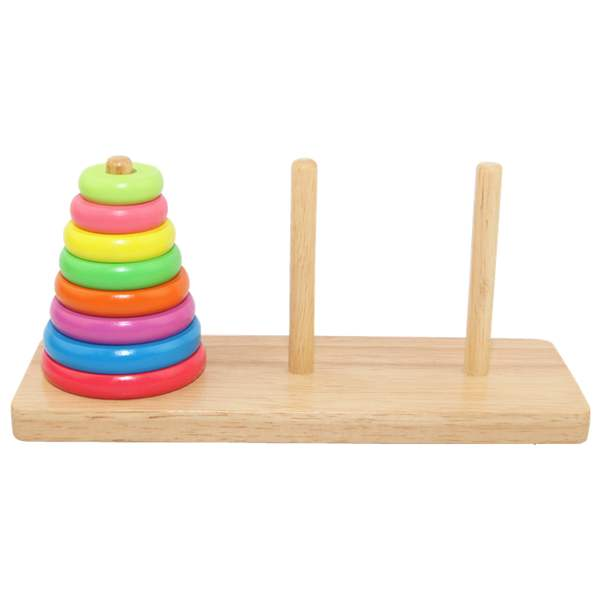
\includegraphics[scale=0.4]{img/C13/13-3/7.png}
\end{figure}

递归算法求解汉诺塔问题:

\begin{enumerate}
	\item 将前n-1个圆盘从A柱借助于C柱搬到B柱。
	\item 将最后一个圆盘直接从A柱搬到C柱。
	\item 将n-1个圆盘从B柱借助于A柱搬到C柱。
\end{enumerate}

\begin{lstlisting}[style=htmlcssjs]
var move = 0;       // 移动次数

/**
 * @brief   汉诺塔算法
 * @note    把 n 个盘子从 src 借助 mid 移到 dst
 * @param   n: 层数
 * @param   src: 起点柱子
 * @param   mid: 临时柱子
 * @param   dst: 目标柱子
 */
function hanoi(n, src, mid, dst) {
    if(n == 1) {
        console.log(n + "号盘:" + src + " -> " + dst);
        move++;
    } else {
        // 把前 n-1 个盘子从 src 借助 dst 移到 mid
        hanoi(n-1, src, dst, mid);
        // 移动第 n 个盘子
        console.log(n + "号盘:" + src + " -> " + dst);
        move++;
        // 把刚才的 n-1 个盘子从 mid 借助 src 移到 dst
        hanoi(n-1, mid, src, dst);
    }
}

hanoi(4, 'A', 'B', 'C');
console.log("步数 ==> " + move);
\end{lstlisting}

\begin{tcolorbox}
	\mybox{运行结果}
	\begin{verbatim}
1号盘:A -> B
2号盘:A -> C
1号盘:B -> C
3号盘:A -> B
1号盘:C -> A
2号盘:C -> B
1号盘:A -> B
4号盘:A -> C
1号盘:B -> C
2号盘:B -> A
1号盘:C -> A
3号盘:B -> C
1号盘:A -> B
2号盘:A -> C
1号盘:B -> C
步数 ==> 15
	\end{verbatim}
\end{tcolorbox}

\newpage

\chapter{事件}

\section{事件}

\subsection{事件(Event)}

JS创建动态页面时,事件是可以被JS侦测到的行为。网页中的每个元素都可以产生某些可以出发JS函数或程序的事件。例如当用户单击或者提交表单数据时,就发生一个鼠标单击事件,需要浏览器做出处理,返回给用户一个结果。

\begin{table}[H]
	\centering
	\setlength{\tabcolsep}{5mm}{
		\begin{tabular}{|c|c|}
			\hline
			\textbf{事件} & \textbf{描述}        \\
			\hline
			onclick       & 鼠标单击事件         \\
			\hline
			onmouseover   & 鼠标经过事件         \\
			\hline
			onmouseout    & 鼠标移开事件         \\
			\hline
			onchange      & 文本框内容改变事件   \\
			\hline
			onselect      & 文本框内容被选中事件 \\
			\hline
			onfocus       & 光标聚集             \\
			\hline
			onblur        & 光标失焦             \\
			\hline
			onload        & 网页导入             \\
			\hline
			onunload      & 关闭网页             \\
			\hline
		\end{tabular}
	}
\end{table}

\newpage

\section{鼠标单击事件}

\subsection{鼠标单击事件onclick}

当在网页上单击鼠标时,就会发生该事件,同时onclick事件调用的程序块就会被执行,onclick通常与按钮一起使用。 \\

\mybox{onclick} \\

\begin{lstlisting}[style=htmlcssjs]
<!DOCTYPE html>
<html lang="en">
<head>
    <meta charset="UTF-8">
    <title>鼠标单击事件onclick</title>
    <script type="text/JavaScript">
        var cnt = 0;
        function feedback() {
            cnt++;
            console.log("我被点击了"+ cnt + "次");
        }
    </script>
</head>
<body>
    <form action="get/post">
        <input type="button" value="点击" onclick="feedback();">
    </form>
</body>
</html>
\end{lstlisting}

\newpage

\section{鼠标经过/移开事件}

\subsection{鼠标经过事件onmouseover}

当鼠标移到一个对象上时,该对象就会触发onmouseover事件,并执行onmouseover事件调用的程序。 \\

\mybox{onmouseover} \\

\begin{lstlisting}[style=htmlcssjs]
<!DOCTYPE html>
<html lang="en">
<head>
    <meta charset="UTF-8">
    <title>鼠标经过事件onmouseover</title>
    <script type="text/JavaScript">
        var cnt = 0;
        function feedback() {
            alert("卸载之前再想想吧...");
        }
    </script>
</head>
<body>
    <form action="get/post">
        <input type="button" value="卸载"
            onmouseover="feedback();">
    </form>
</body>
</html>
\end{lstlisting}

\subsection{鼠标移开事件onmouseout}

当鼠标移开当前对象时,执行onmouseout事件调用的程序。 \\

\mybox{onmouseout} \\

\begin{lstlisting}[style=htmlcssjs]
<!DOCTYPE html>
<html lang="en">
<head>
    <meta charset="UTF-8">
    <title>鼠标移开事件onmouseout</title>
    <script type="text/JavaScript">
        var cnt = 0;
        function feedback() {
            alert("不要离开!只要输入密码,再点击登录就OK啦!");
        }
    </script>
</head>
<body>
    <form action="get/post">
        密码:<input type="password"
                onmouseout="feedback();">
        <input type="button" value="登录">
    </form>
</body>
</html>
\end{lstlisting}

\newpage

\section{光标聚焦/失焦事件}

\subsection{光标聚焦事件onfocus}

当网页中的对象获得聚点时,执行onfocus事件调用的程序。 \\

\mybox{onfocus} \\

\begin{lstlisting}[style=htmlcssjs]
<!DOCTYPE html>
<html lang="en">
<head>
    <meta charset="UTF-8">
    <title>光标聚焦事件onfocus</title>
    <script type="text/JavaScript">
        var flag = true;
        function feedback() {
            if(flag) {
                alert("不要填错啦!");
                flag = false;
            }
        }
    </script>
</head>
<body>
    <form action="get/post">
        密码:<input type="password" onfocus="feedback();">
        <input type="button" value="登录">
    </form>
</body>
</html>
\end{lstlisting}

\subsection{失焦事件onblur}

onblur事件与onfocus事件是相对事件,当光标离开当前获得聚焦对象的时候,就会触发onblur事件,同时执行被调用的程序。 \\

\mybox{onblur} \\

\begin{lstlisting}[style=htmlcssjs]
<!DOCTYPE html>
<html lang="en">
<head>
    <meta charset="UTF-8">
    <title>失焦事件onblur</title>
    <script type="text/JavaScript">
        function feedback() {
            alert("确定输对了再点登录哟!");
        }
    </script>
</head>
<body>
    <form action="get/post">
        密码:<input type="password" onblur="feedback();">
        <input type="button" value="登录">
    </form>
</body>
</html>
\end{lstlisting}

\newpage

\section{内容选中/改变事件}

\subsection{内容选中事件onselect}

当文本框或者文本域中的文本被选中时,触发onselect事件,同时调用的程序就会被执行。 \\

\mybox{onselect} \\

\begin{lstlisting}[style=htmlcssjs]
<!DOCTYPE html>
<html lang="en">
<head>
    <meta charset="UTF-8">
    <title>内容选中事件onselect</title>
    <script type="text/JavaScript">
        function feedback() {
            console.log("文本内容被选中");
        }
    </script>
</head>
<body>
    <form action="get/post">
        <textarea rows="10" cols="30" onselect="feedback();">填写个人信息</textarea>
    </form>
</body>
</html>
\end{lstlisting}

\subsection{内容改变事件onchange}

通过改变文本框的内容可以触发onchange事件,同时执行被调用的程序。 \\

\mybox{onchange} \\

\begin{lstlisting}[style=htmlcssjs]
<!DOCTYPE html>
<html lang="en">
<head>
    <meta charset="UTF-8">
    <title>内容改变事件onchange</title>
    <script type="text/JavaScript">
        function feedback() {
            console.log("文本内容被修改");
        }
    </script>
</head>
<body>
    <form action="get/post">
        <textarea rows="10" cols="30" onchange="feedback();">填写个人信息</textarea>
    </form>
</body>
</html>
\end{lstlisting}

\newpage

\section{加载/卸载事件}

\subsection{加载事件onload}

加载事件会在页面加载完成后立即发生,同时执行被调用的程序。注意,加载事件需要写在<body>内。 \\

\mybox{onload} \\

\begin{lstlisting}[style=htmlcssjs]
<!DOCTYPE html>
<html lang="en">
<head>
    <meta charset="UTF-8">
    <title>加载事件onload</title>
    <script type="text/JavaScript">
        function feedback() {
            alert("页面加载完成");
        }
    </script>
</head>
<body onload="feedback();">
    <p>Hello World!</p>
</body>
</html>
\end{lstlisting}

\subsection{卸载事件onunload}

当用户退出页面时(页面关闭、页面刷新等),就会触发onunload事件,同时执行被调用的程序。注意,不同浏览器对onunload事件的支持不同。

\newpage

\chapter{对象}

\section{对象}

\subsection{对象(Object)}

JS中的所有事物都是对象,如字符串、数值、数组、函数等,每个对象带有属性和方法。对象的属性反映了该对象的某些特定性质,如字符串的长度、图像的长宽等,对象的方法指的是能够在对象上执行的动作,如表单的提交、时间的获取等。 \\

JS提供了多个内建对象,如String、Date、Array等,使用对象前需要先使用new关键字进行定义。 \\

\mybox{访问对象属性} \\

\begin{lstlisting}[style=htmlcssjs]
var arr = new Array(1, 2, 3, 4, 5);
console.log(arr.length);
\end{lstlisting}

\begin{tcolorbox}
	\mybox{运行结果}
	\begin{verbatim}
5
	\end{verbatim}
\end{tcolorbox}

\vspace{0.5cm}

\mybox{访问对象方法} \\

\begin{lstlisting}[style=htmlcssjs]
var str = "Hello World";
console.log(str.toUpperCase());
\end{lstlisting}

\begin{tcolorbox}
	\mybox{运行结果}
	\begin{verbatim}
HELLO WORLD
	\end{verbatim}
\end{tcolorbox}

\newpage

\section{Date}

\subsection{Date}

Date对象可以存储任意一个日期,并且可以精确到毫秒数($ 1 / 1000 $秒)。使用默认构造函数创建的日期对象有初始值,为当前电脑系统时间。 \\

\mybox{定义Date对象} \\

\begin{lstlisting}[style=htmlcssjs]
var date1 = new Date();
console.log(date1);

var date2 = new Date(2021, 3, 19);      //此处月份从0开始
console.log(date2);
\end{lstlisting}

\begin{tcolorbox}
	\mybox{运行结果}
	\begin{verbatim}
2021-03-19T05:09:47.713Z
2021-04-18T16:00:00.000Z
	\end{verbatim}
\end{tcolorbox}

\begin{table}[H]
	\centering
	\setlength{\tabcolsep}{5mm}{
		\begin{tabular}{|l|l|}
			\hline
			\textbf{方法名称}             & \textbf{描述}                      \\
			\hline
			getDate() / setDate()         & 返回/设置日期                      \\
			\hline
			getFullYear() / setFullYear() & 返回/设置年份,用四位数表示        \\
			\hline
			getYear() / setYear()         & 返回/设置年份                      \\
			\hline
			getMonth() / setMonth()       & 返回/设置月份,月份从0开始         \\
			\hline
			getHours() / setHours()       & 返回/设置小时,24小时制            \\
			\hline
			getMinutes() / setMinutes()   & 返回/设置分钟数                    \\
			\hline
			getSeconds() / setSeconds()   & 返回/设置秒钟数                    \\
			\hline
			getTime() / setTime()         & 返回/设置时间(毫秒为单位)        \\
			\hline
			getDay()                      & 返回0-6的数字表示星期,0表示星期天 \\
			\hline
		\end{tabular}
	}
	\caption{Date方法}
\end{table}

\mybox{获取今日星期} \\

\begin{lstlisting}[style=htmlcssjs]
var date = new Date();
var weekday = [
    "星期天",
    "星期一",
    "星期二",
    "星期三",
    "星期四",
    "星期五",
    "星期六"
];
console.log("今天是" + weekday[date.getDay()]);
\end{lstlisting}

\begin{tcolorbox}
	\mybox{运行结果}
	\begin{verbatim}
今天是星期五
	\end{verbatim}
\end{tcolorbox}

\newpage

\section{String}

\subsection{计算字符串长度}

定义String对象后就可以访问它的属性和方法。 \\

\mybox{计算字符串长度} \\

\begin{lstlisting}[style=htmlcssjs]
var str = "Hello World!"
console.log(str.length);
\end{lstlisting}

\begin{tcolorbox}
	\mybox{运行结果}
	\begin{verbatim}
12
	\end{verbatim}
\end{tcolorbox}

\subsection{大小写转换}

使用String对象的toUpperCase()和toLowerCase()可以将字符串进行大小写字母转换。 \\

\mybox{大小写字母转换} \\

\begin{lstlisting}[style=htmlcssjs]
var str = "Hello World!"
console.log(str.toUpperCase());
console.log(str.toLowerCase());
\end{lstlisting}

\begin{tcolorbox}
	\mybox{运行结果}
	\begin{verbatim}
HELLO WORLD!
hello world!
	\end{verbatim}
\end{tcolorbox}

\subsection{返回指定的字符}

使用charAt()可返回指定位置的字符,返回的字符是长度为1的字符串。 \\

\mybox{charAt()} \\

\begin{lstlisting}[style=htmlcssjs]
var str = "Hello World!"
console.log(str.charAt(6));
\end{lstlisting}

\begin{tcolorbox}
	\mybox{运行结果}
	\begin{verbatim}
W
	\end{verbatim}
\end{tcolorbox}

\subsection{返回指定的字符串首次出现的位置}

indexOf()可以返回某个指定的字符串值在字符串中首次出现的位置。 \\

\begin{lstlisting}[style=htmlcssjs]
stringObj.indexOf(substring, startPos);
\end{lstlisting}

该方法将从头到尾地检索字符串,检查是否含有需检索的子串。参数startPos为可选参数,用于规定开始查找的位置,如果没有设置此参数将从头开始查找。如果找到了子串,在返回子串的第一次出现位置。如果要检索的字符串值没有出现,则该方法返回-1。 \\

\mybox{indexOf()} \\

\begin{lstlisting}[style=htmlcssjs]
var str = "Hello World!";
console.log(str.indexOf("Hell"));
console.log(str.indexOf("o", 6));
console.log(str.indexOf("JS"));
\end{lstlisting}

\begin{tcolorbox}
	\mybox{运行结果}
	\begin{verbatim}
0
7
-1
	\end{verbatim}
\end{tcolorbox}

\subsection{字符串分割}

split()可以将字符串分割为字符串数组,并返回此数组。 \\

\begin{lstlisting}[style=htmlcssjs]
stringObj.split(separator, limit);
\end{lstlisting}

其中参数separator必选,用于指定将字符串按某个字符切割成若干个子字符串,并以数组的形式返回。参数limit可选,用于指定分隔的次数。如果把空字符串作为separator,那么字符串的每个字符之间都会被分隔。 \\

\mybox{split()} \\

\begin{lstlisting}[style=htmlcssjs]
var str = "hello HTML hello CSS hello JavaScript";
console.log(str.split(" "));
console.log(str.split(" ", 4));
\end{lstlisting}

\begin{tcolorbox}
	\mybox{运行结果}
	\begin{verbatim}
["hello", "HTML", "hello", "CSS", "hello", "JavaScript"]
["hello", "HTML", "hello", "CSS"]
	\end{verbatim}
\end{tcolorbox}

\subsection{提取字符串}

substring()用于提取字符串中介于两个指定下标之间的字符。 \\

\begin{lstlisting}[style=htmlcssjs]
stringObj.substring(startPos, stopPos);
\end{lstlisting}

该方法返回的内容是从startPos开始到stopPos - 1处的所有内容,其长度为stopPos - startPos。如果startPos和stopPos相等,那么返回的就是一个空串(长度为0的字符串)。如果startPos比stopPos大,那么该方法在提取子串之间会先交换这两个参数。 \\

\mybox{substring()} \\

\begin{lstlisting}[style=htmlcssjs]
var str = "HelloWorld";
console.log(str.substring(2, 8));
console.log(str.substring(3, 3));
console.log(str.substring(7, 3));
\end{lstlisting}

\begin{tcolorbox}
	\mybox{运行结果}
	\begin{verbatim}
lloWor

loWo
	\end{verbatim}
\end{tcolorbox}

\subsection{提取指定数目的字符}

substr()用于从字符串中提取从startPos位置开始的指定数目的字符串。 \\

\begin{lstlisting}[style=htmlcssjs]
stringObj.substr(startPos, length);
\end{lstlisting}

如果参数startPos是负数,则从字符串的尾部开始算起,如果startPos为负数且绝对值大于字符串长度,则startPos会被视为0。 \\

\mybox{substr()} \\

\begin{lstlisting}[style=htmlcssjs]
var str = "HelloWorld";
console.log(str.substr(2, 3));
console.log(str.substr(-5, 4));
\end{lstlisting}

\begin{tcolorbox}
	\mybox{运行结果}
	\begin{verbatim}
llo
Worl
	\end{verbatim}
\end{tcolorbox}

\newpage

\section{Math}

\subsection{Math}

Math对象提供对数据的数学计算。需要注意的是,Math对象是一个固有的对象,无需创建它,直接把Math作为对象使用就可以调用其所有属性和方法,这是它与其它对象的区别。

\begin{table}[H]
	\centering
	\setlength{\tabcolsep}{5mm}{
		\begin{tabular}{|c|l|}
			\hline
			\textbf{属性} & \textbf{描述}                                          \\
			\hline
			E             & 返回算术常量$ e $,即自然对数的底数(约等于$ 2.718 $) \\
			\hline
			LN2           & 返回$ 2 $的自然对数(约等于$ 0.693 $)                 \\
			\hline
			LN10          & 返回$ 10 $的自然对数(约等于$ 2.302 $)                \\
			\hline
			LOG2E         & 返回以$ 2 $为底$ e $的对数(约等于$ 1.442 $)          \\
			\hline
			LOG10E        & 返回以$ 10 $为底$ e $的对数(约等于$ 0.434 $)         \\
			\hline
			PI            & 返回圆周率(约等于$ 3.14159 $)                        \\
			\hline
			SQRT1\_2      & 返回$ 2 $的平方根的倒数(约等于$ 0.707 $)             \\
			\hline
			SQRT2         & 返回$ 2 $的平方根(约等于$ 1.414 $)                   \\
			\hline
		\end{tabular}
	}
	\caption{Math属性}
\end{table}

\begin{table}[H]
	\centering
	\setlength{\tabcolsep}{5mm}{
		\begin{tabular}{|c|l|}
			\hline
			\textbf{方法} & \textbf{描述}                    \\
			\hline
			sin(x)        & 返回$ x $的正弦                  \\
			\hline
			cos(x)        & 返回$ x $的余弦                  \\
			\hline
			tan(x)        & 返回$ x $的正切                  \\
			\hline
			acos(x)       & 返回$ x $的反余弦值              \\
			\hline
			asin(x)       & 返回$ x $的反正弦值              \\
			\hline
			atan(x)       & 返回$ x $的反正切值              \\
			\hline
			ceil(x)       & 对$ x $进行上取整                \\
			\hline
			floor(x)      & 对$ x $进行下取整                \\
			\hline
			abs(x)        & 返回$ x $的绝对值                \\
			\hline
			exp(x)        & 返回$ e $的$ x $次幂             \\
			\hline
			log(x)        & 返回$ x $的自然对数(底为$ e $) \\
			\hline
			pow(x, y)     & 返回$ x $的$ y $次幂             \\
			\hline
			max(x, y)     & 返回$ x $和$ y $中的最大值       \\
			\hline
			min(x, y)     & 返回$ x $和$ y $中的最小值       \\
			\hline
			round(x)      & 返回$ x $的四舍五入最接近的整数  \\
			\hline
			sqrt(x)       & 返回$ x $的平方根                \\
			\hline
			random()      & 返回$ 0 \sim 1 $之间的随机数     \\
			\hline
		\end{tabular}
	}
	\caption{Math方法}
\end{table}

\newpage

\chapter{浏览器对象模型BOM}

\section{window对象}

\subsection{window对象}

window对象是浏览器对象模型BOM(Browser Object Model)的核心。

\begin{table}[H]
	\centering
	\setlength{\tabcolsep}{5mm}{
		\begin{tabular}{|c|l|}
			\hline
			\textbf{方法} & \textbf{描述}                                  \\
			\hline
			alert()       & 显示带有一段消息和一个确认按钮的警告框         \\
			\hline
			prompt()      & 显示可提示用户输入的对话框                     \\
			\hline
			confirm()     & 显示带有一段消息以及确认按钮和取消按钮的对话框 \\
			\hline
			open()        & 打开一个新的浏览器窗口或查找一个已命名的窗口   \\
			\hline
			close()       & 关闭浏览器窗口                                 \\
			\hline
			print()       & 打印当前窗口的内容                             \\
			\hline
			focus()       & 把焦点给与一个窗口                             \\
			\hline
			blur()        & 把焦点从顶层窗口移开                           \\
			\hline
			moveBy()      & 可相对窗口的当前坐标把它移动指定的像素         \\
			\hline
			moveTo()      & 把窗口的左上角移动到一个指定的坐标             \\
			\hline
			resizeTo()    & 把窗口的大小调整到指定的宽度和高度             \\
			\hline
			scrollBy()    & 按照指定的像素值来滚动内容                     \\
			\hline
			scrollTo()    & 把内容滚动到指定的坐标                         \\
			\hline
		\end{tabular}
	}
	\caption{window方法}
\end{table}

\newpage

\section{计时器}

\subsection{计时器}

在JS中,可以在设定的时间间隔之后执行代码,而不是在函数被调用后立即执行。 \\

计时器的类型分为2种:

\begin{enumerate}
	\item 一次性计时器:仅在指定的延迟时间之后触发一次。
	\item 间隔性触发计时器:每隔一定的时间间隔就触发一次。
\end{enumerate}

\begin{table}[H]
	\centering
	\setlength{\tabcolsep}{5mm}{
		\begin{tabular}{|c|l|}
			\hline
			\textbf{方法}   & \textbf{描述}                  \\
			\hline
			setTimeout()    & 在指定的延迟时间之后来执行代码 \\
			\hline
			clearTimeout()  & 取消setTimeout()的设置         \\
			\hline
			setInterval()   & 每隔指定的时间执行代码         \\
			\hline
			clearInterval() & 取消setInterval()的设置        \\
			\hline
		\end{tabular}
	}
	\caption{计时器方法}
\end{table}

\subsection{setTimeout()}

setTimeout()计时器,在载入后延迟指定时间后,去执行一次表达式,仅执行一次。 \\

\begin{lstlisting}[style=htmlcssjs]
setTimeout(expr, timeout);
\end{lstlisting}

\begin{itemize}
	\item expr:要调用的函数或要执行的代码串。
	\item timeout:在执行代码前需等待的时间,以毫秒为单位(1s = 1000ms)。
\end{itemize}

\begin{lstlisting}[style=htmlcssjs]
// 网页打开2秒后弹出提示框
setTimeout("alert('Welcome')", 2000);
\end{lstlisting}

clearTimeout()和setTimeout()一起使用,用于停止计时器。 \\

\begin{lstlisting}[style=htmlcssjs]
clearTimeout(id_of_setTimeout);
\end{lstlisting}

id\_of\_setTimeout:setTimeout()返回的ID值,该值标识要取消的延迟执行代码块。 \\

\mybox{计数器}

\begin{lstlisting}[style=htmlcssjs, title=counter.html]
<!DOCTYPE html>
<html lang="en">
<head>
    <meta charset="UTF-8">
    <title>计数器</title>
    <script src="counter.js"></script>
</head>
<body>
    <form action="get/post">
        <input type="text" id="num">
        <input type="button" value="stop" onclick="stopCount();">
    </form>
</body>
</html>
\end{lstlisting}

\begin{lstlisting}[style=htmlcssjs, title=counter.js]
var cnt = 0;        // 计数
var counter;        // 计数器

/**
 * 每隔1000毫秒计数加1
 */
function count() {
    document.getElementById('num').value = cnt;
    cnt++;
    counter = setTimeout(count, 1000);
}

/**
 * 停止计数器
 */
function stopCount() {
    clearTimeout(counter);
}

setTimeout(count, 1000);        // 启动计数器
\end{lstlisting}

\subsection{setInterval()}

setInterval()在执行时,从载入页面后每隔指定的时间执行代码。 \\

\begin{lstlisting}[style=htmlcssjs]
setInterval(expr, interval);
\end{lstlisting}

\begin{itemize}
	\item expr:要调用的函数或要执行的代码串。
	\item interval:周期性执行或调用表达式之间的时间间隔,以毫秒为单位(1s = 1000ms)。
\end{itemize}

clearInterval()可取消由setInterval()设置的交互时间。 \\

\begin{lstlisting}[style=htmlcssjs]
clearInterval(id_of_setInterval);
\end{lstlisting}

id\_of\_setInterval:setInterval()返回的ID值。 \\

\mybox{实时显示当前时间}

\begin{lstlisting}[style=htmlcssjs, title=current\_time.html]
<!DOCTYPE html>
<html lang="en">
<head>
    <meta charset="UTF-8">
    <title>显示当前时间</title>
    <script src="current_time.js"></script>
</head>
<body>
    <form action="get/post">
        <input type="text" id="time" size="50">
    </form>
</body>
</html>
\end{lstlisting}

\begin{lstlisting}[style=htmlcssjs, title=current\_time.js]
// function clock() {
//     var date = new Date();
//     document.getElementById("time").value = date;
// }

// setInterval(clock, 1000);

// 箭头函数
setInterval(() => {
    var date = new Date();
    document.getElementById("time").value = date;
}, 1000);
\end{lstlisting}

\newpage

\section{Screen对象}

\subsection{Screen对象}

Screen对象用于获取用户的屏幕信息。window.screen对象在编写时可以不使用window前缀。

\begin{table}[H]
	\centering
	\setlength{\tabcolsep}{5mm}{
		\begin{tabular}{|c|l|}
			\hline
			\textbf{属性} & \textbf{描述}                    \\
			\hline
			availHeight   & 窗口可以使用的屏幕高度,单位像素 \\
			\hline
			availWidth    & 窗口可以使用的屏幕宽度,单位像素 \\
			\hline
			height        & 屏幕的高度,单位像素             \\
			\hline
			width         & 屏幕的宽度,单位像素             \\
			\hline
		\end{tabular}
	}
	\caption{Screen属性}
\end{table}

screen.availWidth和screen.availHeight属性返回访问者屏幕的宽度和高度,单位为像素,减去界面特性,比如任务栏等。不同系统的任务栏默认高度不一样,及任务栏的位置可在屏幕上下左右任何位置,所以有可能可用宽度和高度不一样。 \\

\mybox{屏幕信息} \\

\begin{lstlisting}[style=htmlcssjs]
<!DOCTYPE html>
<html lang="en">
<head>
    <meta charset="UTF-8">
    <title>屏幕信息</title>
    <script type="text/JavaScript">
        console.log("屏幕分辨率:"
					+ screen.width + "*"
					+ screen.height)
        console.log("屏幕可用宽高:"
					+ screen.availWidth + "*"
					+ screen.availHeight);
    </script>
</head>
<body>

</body>
</html>
\end{lstlisting}

\newpage

\chapter{文档对象模型DOM}

\section{DOM}

\subsection{DOM(Document Object Model)}

\begin{figure}[H]
	\centering
	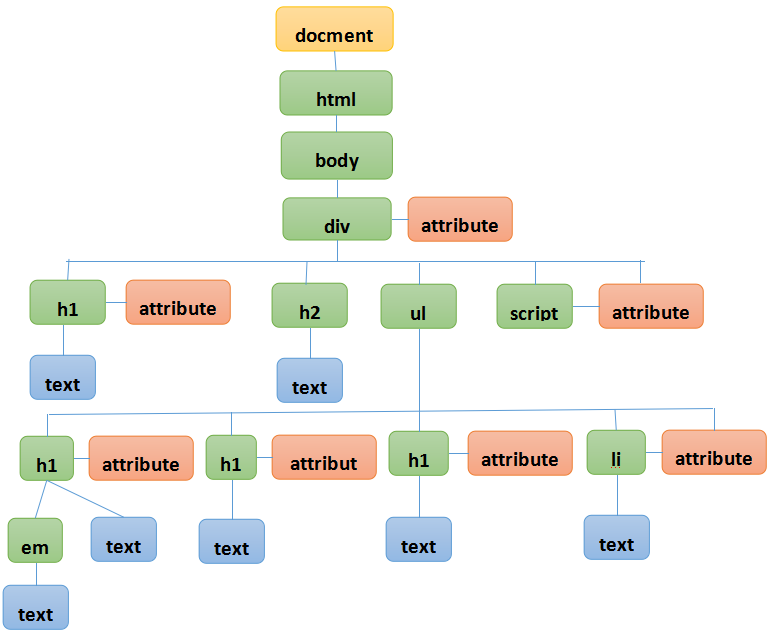
\includegraphics[scale=0.8]{img/C17/17-1/1.png}
\end{figure}

\newpage

\section{获取结点对象}

\subsection{getElementById()}

getElementById()可返回拥有指定ID的第一个对象的引用。如果没有指定ID的元素则返回null,如果存在多个指定ID的元素则返回第一个。 \\

\mybox{定时变换颜色}

\begin{lstlisting}[style=htmlcssjs, title=random\_color.html]
<!DOCTYPE html>
<html lang="en">
<head>
    <meta charset="UTF-8">
    <title>随机颜色</title>
    <script src="random_color.js"></script>
</head>
<body>
    <div id="square" style="width: 100px; height: 100px"></div>
</body>
</html>
\end{lstlisting}

\begin{lstlisting}[style=htmlcssjs, title=random\_color.js]
/**
 * 随机生成RGB颜色代码
 * @returns rgb颜色
 */
function randomRGB() {
    var r = Math.floor(Math.random() * 256);
    var g = Math.floor(Math.random() * 256);
    var b = Math.floor(Math.random() * 256);
    return "rgb(" + r + ", " + g + ", " + b + ")";
}

/**
 * 获取元素结点,设置背景颜色
 */
function changeColor() {
    var obj = document.getElementById("square");
    obj.style.background = randomRGB();
}

// 每隔300ms改变颜色
setInterval(function () {
    changeColor();
}, 300);
\end{lstlisting}

\subsection{getElementsByClassName()}

getElementByClassName()返回文档中所有指定类名的元素集合,作为NodeList对象。NodeList对象代表一个有顺序的结点列表,可以通过索引来访问列表中的结点。使用NodeList的length属性可以确定指定类名的元素个数,并循环各个元素来获取某个元素。 \\

\begin{lstlisting}[style=htmlcssjs]
document.getElementsByClassName(className);
\end{lstlisting}

\subsection{getElementByName()}

getElementByName()返回带有指定名称的结点对象的集合。 \\

\begin{lstlisting}[style=htmlcssjs]
document.getElementsByName(name);
\end{lstlisting}

getElementByName()通过元素name属性查询元素,文档中的name属性可能不唯一,所以getElementByName()返回的是元素的数组,而不是一个元素。

\subsection{getElementsByTagName()}

getElementsByTagName()返回带有指定标签名的结点对象的集合,返回元素的顺序是它们在文档中的顺序。 \\

\begin{lstlisting}[style=htmlcssjs]
document.getElementsByTagName(tagName);
\end{lstlisting}

\newpage

\section{结点操作}

\subsection{结点属性}

getAttribute()可以通过元素结点的属性名称获取属性的值。 \\

\begin{lstlisting}[style=htmlcssjs]
elementNode.getAttribute(name);
\end{lstlisting}

其中,elementNode可以使用getElementById()、getElementsByTagName()等方法获取到元素结点,参数name为需要查询的元素结点的属性名称。 \\

setAttribute()可以增加一个指定名称和值的新属性,或者把一个现有的属性设定为指定的值。 \\

\begin{lstlisting}[style=htmlcssjs]
elementNode.setAttribute(name, value);
\end{lstlisting}

\vspace{0.5cm}

\mybox{设置结点属性值}

\begin{lstlisting}[style=htmlcssjs, title=getAttribute.html]
<!DOCTYPE html>
<html lang="en">
<head>
    <meta charset="UTF-8">
    <title>设置结点属性</title>
    <script src="getAttribute.js"></script>
</head>
<body>
    <a class="link" href="https://www.baidu.com">百度</a>
    <a class="link" href="https://www.bilibili.com">哔哩哔哩</a>
</body>
</html>
\end{lstlisting}

\begin{lstlisting}[style=htmlcssjs, title=getAttribute.js]
window.onload = function() {
    var links = document.getElementsByClassName("link");
    for(var i = 0; i < links.length; i++) {
        console.log(links[i].getAttribute("href"));
        links[i].setAttribute("target", "_blank");
    }
};
\end{lstlisting}

\begin{tcolorbox}
	\mybox{运行结果}
	\begin{verbatim}
https://www.baidu.com
https://www.bilibili.com
	\end{verbatim}
\end{tcolorbox}

\subsection{结点操作}

createElement()用于创建结点元素,此方法可返回一个Element对象。 \\

createElement()要与appendChild()或insertBefore()联合使用,将元素显示在页面中。 \\

\begin{lstlisting}[style=htmlcssjs]
document.createElement(tagName);
\end{lstlisting}

appendChild()用于在指定结点的最后一个子结点列表之后添加一个新的子结点。 \\

\begin{lstlisting}[style=htmlcssjs]
elementNode.appendChild(newNode);
\end{lstlisting}

insertBefore()用于在已有的子结点前插入一个新的子结点。 \\

\begin{lstlisting}[style=htmlcssjs]
elementNode.insertBefore(newNode, node);
\end{lstlisting}

removeChild()用于从子结点列表中删除某个结点,如删除成功返回被删除的结点,如失败则返回null。 \\

\begin{lstlisting}[style=htmlcssjs]
elementNode.removeChild(node);
\end{lstlisting}

replaceChild():实现子结点的替换,返回被替换对象的引用。当oldNode被替换时,所有与之相关的属性内容都将被移出。 \\

\begin{lstlisting}[style=htmlcssjs]
elementNode.replaceChild(newNode, oldNode);
\end{lstlisting}